% OMEGA_NOTE.tex -- Gomez's compound graphs Omega H_q and the D = 8 entries of the bipartite table.
% Build: tectonic OMEGA_NOTE.tex  (XeTeX; uses fontspec, DejaVu Sans Mono for the Lean block, TikZ).
% Markdown version: ../OMEGA_NOTE.md (same content).
\documentclass[11pt]{amsart}
\usepackage{amsmath,amssymb,amsthm}
\usepackage[no-math]{fontspec}
\setmonofont{DejaVuSansMono.ttf}[Scale=0.78]
\usepackage{enumitem}
\usepackage{booktabs}
\usepackage{array}
\usepackage[margin=1in]{geometry}
\usepackage{tikz}
\usetikzlibrary{calc}
\usepackage[hidelinks]{hyperref}
\usepackage{xurl}
\newcommand{\file}[1]{\nolinkurl{#1}}
\usepackage{fancyvrb}

\setlist{itemsep=2pt,topsep=3pt}
\renewcommand{\arraystretch}{1.12}

\theoremstyle{plain}
\newtheorem{theorem}{Theorem}
\newtheorem{lemma}{Lemma}[section]
\newtheorem{corollary}[lemma]{Corollary}
\newtheorem{fact}[lemma]{Fact}
\newtheorem{computer}{Computer-checked}
\renewcommand{\thecomputer}{C\arabic{computer}}
\newtheorem{heuristic}{Heuristic}
\renewcommand{\theheuristic}{H\arabic{heuristic}}
\theoremstyle{definition}
\newtheorem{definition}[lemma]{Definition}
\newtheorem*{example}{Example}
\theoremstyle{remark}
\newtheorem*{remark}{Remark}

\newcommand{\F}{\mathbb{F}}
\newcommand{\PG}{\mathrm{PG}}
\newcommand{\Q}{\mathsf{Q}}
\newcommand{\opp}{\mathrm{opp}}
\newcommand{\Perp}{\mathrm{Perp}}
\newcommand{\Aut}{\mathrm{Aut}}
\newcommand{\GG}{\mathrm{G}_2}
\newcommand{\cP}{\mathcal{P}}
\newcommand{\cL}{\mathcal{L}}
\newcommand{\bk}[1]{\overline{#1}}
\newcommand{\Om}{\Omega}
\newcommand{\ip}{\perp}
\newcommand{\pP}{P}  % point set
\newcommand{\lL}{L}  % line set

\title[Gómez's $\Om H_q$ and the diameter-8 entries]{Gómez's compound graphs $\Om H_q$ and the diameter-8 entries\\ of the bipartite degree--diameter table}
\author{Degree--diameter lab}
\address{github.com/dogaozden/degree-diameter (Claude Code sessions coordinated by Doğa Özden)}
\date{Draft, 28 October 2026, for Gabriela Araujo-Pardo and Ignacio López. Replaces the one-page note of 26 October.}

\begin{document}

\begin{abstract}
Six diameter-8 entries of the bipartite degree--diameter table, credited to Delorme, Gómez and Quisquater, are the orders of
the compound graphs $\Om H_q$ of Gómez's 1986 thesis ($q = 7, 8, 9, 11, 11, 13$), which the thesis states to have diameter
$\le 8$ without proof. We show that, as defined (every copy of the hexagon carries the same labels), $\Om H_q$ has
diameter at least $9$ under every reading of the figures (Theorems~\ref{thm:one} and~\ref{thm:two}; Theorem~\ref{thm:one}
is also formalised in Lean). Giving each copy its own labelling is the natural repair; we show that it fails for every
$q \ge 7$ whenever the labelling respects the geometry of the hexagon (Theorems~\ref{thm:geo8} and~\ref{thm:geo7}).
Arbitrary relabellings remain open for $q \ge 4$; at $q = 2, 3$ they do give diameter~$8$.
\end{abstract}

\maketitle

\noindent\textbf{Labels.} Every claim carries one of these labels.
\begin{itemize}[leftmargin=1.5em]
\item \textbf{Theorem}: proved by hand in this note, with a complete proof. Lemmas and corollaries proved here carry the tag
  ``Theorem'' in their heading. \emph{Theorem (computer-assisted)}: the proof is complete except for one named
  Computer-checked statement.
\item \textbf{Computer-checked}: a statement about finite data, with the programs and logs that check it (\S\ref{sec:sources}).
  ``Twice'' means by two programs written separately, in different sessions, sharing no code.
\item \textbf{Heuristic}: an argument with a named gap. It is not a proof.
\item \textbf{Fact}: a standard result, quoted with a reference.
\end{itemize}
File paths refer to the repository; the branch of each source is listed in \S\ref{sec:sources}.

\section*{Summary}\label{sec:summary}

In the 2013 survey table \cite[Table 4]{MS13}, reproduced on the CombinatoricsWiki \cite{CW}, six entries with $D = 8$
are the orders of Gómez's graphs $\Om H_q$ \cite[\S2.9.3, values on p.~46]{Go86}. Here $H(q)$ is the split Cayley
hexagon, its incidence graph has $N_1 = 2N$ vertices with $N = (q^6-1)/(q-1)$, and $q + 3 = 2\alpha + \beta$ with
$\beta \in \{0,1\}$:
\begin{center}\small
\begin{tabular}{@{}lrlrrrrr@{}}
\toprule
cell & table value & graph & $q$ & $\alpha$ & copies & hubs & order $5(\alpha+1)N_1$\\
\midrule
$(10,8)$ & 1,176,480 & $\Om H_7$ & 7 & 5 & 25 & 196,080 & 1,176,480\\
$(11,8)$ & 2,246,940 & $\Om H_8$ & 8 & 5 & 25 & 374,490 & 2,246,940\\
$(12,8)$ & 4,650,100 & $\Om H_9$ & 9 & 6 & 30 & 664,300 & 4,650,100\\
$(14,8)$ & 14,172,480 & $\Om H_{11}$ & 11 & 7 & 35 & 1,771,560 & 14,172,480\\
$(15,8)$ & 14,172,480 & $\Om H_{11}$ (reused) & 11 & 7 & 35 & 1,771,560 & 14,172,480\\
$(16,8)$ & 36,201,060 & $\Om H_{13}$ & 13 & 8 & 40 & 4,022,340 & 36,201,060\\
\bottomrule
\end{tabular}
\end{center}
The thesis states $D \le D_1 + 2 = 8$ and gives no proof. The paper the table cites \cite{DGQ} was never published, as
far as we could find.
\begin{enumerate}[leftmargin=1.5em]
\item \textbf{Theorem~\ref{thm:one} (one label; also in Lean).} If a new vertex is joined only to copies of one vertex $t$
  of $B_1$ and misses a copy, it is at distance $\ge d_{B_1}(t,v) + 3$ from the copy of $v$ in the missed copy. In one
  reading of the figures this gives $\operatorname{diam} \Om H_q \ge 9$ for every $q$ and every pairing of labels.
\item \textbf{Theorem~\ref{thm:two} (two labels, $q \ge 7$).} For the thesis's labelling and every reading of the
  figures, every hub has at least $q^5 - 5q^4 - 8q^3 - 12q^2 - 16q - 10$ vertices at distance $\ge 9$ in every copy it
  misses. This covers the six table entries. By computer, $\Om H_7$ and $\Om H_9$ have diameter exactly~$9$.
\item \textbf{Theorems~\ref{thm:geo8} and~\ref{thm:geo7} (geometric relabellings, $q \ge 7$).} Give every copy its own
  labelling, and call it geometric if every transfer map between two copies met by one hub class is induced by an
  automorphism of the incidence graph of $H(q)$. For every $q \ge 7$, every geometric labelling, every reading and every
  mix of block types, the diameter is still $\ge 9$. For $q \ge 10$ the proof is by hand; for $q = 8, 9$ it uses a
  computer count of route words (\ref{cc:routes}); for $q = 7$ it also uses Bonferroni inequalities and a
  character-sum bound.
\item \textbf{Open (\S\ref{sec:open}).} Arbitrary (non-geometric) relabellings for every $q \ge 4$ (at $q = 2, 3$ they
  give diameter $8$); labellings chosen per hub class and copy; other wirings; the geometric class at $q \le 5$.
\item \textbf{What can be claimed (\S\ref{sec:claims}).} The six entries have no checkable graph of diameter~$8$. We do
  not claim that no $(\Delta, 8)$ graph of these orders exists.
\end{enumerate}

\section{The split Cayley hexagon}\label{sec:hexagon}

\subsection{Coordinates}
We use the model of our diameter-7 note \cite[\S1.1]{OD7}, which all of the lab's generators use. Let $q$ be a prime
power, $\F = \F_q$ and $V = \F^7$ with coordinates $(X_0, \dots, X_6)$. Put
\begin{align*}
\Q(X) &= X_0X_4 + X_1X_5 + X_2X_6 - X_3^2,\\
b(X,Y) &= \Q(X+Y) - \Q(X) - \Q(Y) = X_0Y_4 + X_4Y_0 + X_1Y_5 + X_5Y_1 + X_2Y_6 + X_6Y_2 - 2X_3Y_3 .
\end{align*}
The parabolic quadric $Q(6,q)$ is the set of points $\langle x\rangle$ of $\PG(6,q)$ with $\Q(x) = 0$. Two points
$\langle x\rangle, \langle y\rangle$ of $Q(6,q)$ are \emph{perpendicular}, $x \ip y$, if $b(x,y) = 0$; since
$\Q(\lambda x + \mu y) = \lambda\mu\, b(x,y)$, this means that the line $xy$ lies on $Q(6,q)$. We write $x^\perp$ for
the hyperplane $b(x,\cdot) = 0$.

The split Cayley hexagon $H = H(q)$ \cite{Ti59}, \cite[\S2.4]{VM98} has
\begin{itemize}[leftmargin=1.5em]
\item points: the set $\pP$ of all $N = (q^6-1)/(q-1)$ points of $Q(6,q)$;
\item lines: the set $\lL$ of the lines of $Q(6,q)$ whose Grassmann coordinates $p_{ij} = x_iy_j - x_jy_i$ (for two
  spanning points $x, y$) satisfy
  \[ p_{12} = p_{34},\quad p_{54} = p_{32},\quad p_{20} = p_{35},\quad p_{65} = p_{30},\quad p_{01} = p_{36},\quad p_{46} = p_{31}; \]
\item incidence: containment.
\end{itemize}
For example, the $q+1$ lines through $e_0 = (1,0,\dots,0)$ are $\langle e_0, \lambda e_5 + \mu e_6\rangle$,
$(\lambda:\mu) \in \PG(1,q)$; they lie in the totally singular plane $\langle e_0, e_5, e_6\rangle$. The incidence graph
$I = I(q)$ has vertex set $\pP \cup \lL$ ($2N$ vertices). We write $d$ for its distance,
$S_i(z) = \{u : d(z,u) = i\}$, $B(z,R) = \{u : d(z,u) \le R\}$, and $\opp(z) = S_6(z)$ (the elements \emph{opposite}~$z$).

\begin{fact}[{\cite{Ti59}, \cite[\S2.4]{VM98}}]\label{fact:gh}
$H(q)$ is a generalized hexagon of order $(q,q)$: $I$ is connected, bipartite, $(q+1)$-regular, of diameter $6$ and
girth $12$. The lines of $H(q)$ through a point $x$ are the lines through $x$ of a totally singular plane
$\pi_x \subset x^\perp$.
\end{fact}

\begin{fact}[{\cite{Ti59}, \cite{VM98}}]\label{fact:aut}
The automorphisms of $I$ fixing $\pP$ are the collineations of $H(q)$; they form $\GG(q) \rtimes \Aut(\F_q)$ and are
induced by semilinear maps of $V$ preserving $\Q$. For $q$ prime every collineation is induced by a linear map in
$\GG(q) \le \mathrm{SO}(7,q)$. For example, for $A \in \mathrm{SL}(3,q)$ the map $(v, a, w) \mapsto (Av, a, A^{-T}w)$,
where $x = (v,a,w)$ with $v = (x_0,x_1,x_2)$, $a = x_3$, $w = (x_4,x_5,x_6)$, lies in $\GG(q)$. An automorphism of $I$
exchanging $\pP$ and $\lL$ (a \emph{duality}) exists if and only if $q$ is a power of~$3$.
\end{fact}

\begin{fact}[eigenvalues in $\GG$]\label{fact:eig}
For $h \in \GG(q)$ acting on $V$, the eigenvalues of $h$ in $\overline{\F}_q$, with multiplicity, are
$1, x_1^{\pm1}, x_2^{\pm1}, x_3^{\pm1}$ with $x_1x_2x_3 = 1$. (The semisimple part of $h$ is conjugate over
$\overline{\F}_q$ into the maximal torus $\operatorname{diag}(a,b,c,1,a^{-1},b^{-1},c^{-1})$, $abc = 1$, of the subgroup
$\mathrm{SL}(3)$ above, and $h$ has the characteristic polynomial of its semisimple part.)
\end{fact}

\subsection{Distances}

\begin{lemma}[Theorem; distance profile]\label{lem:profile}
Let $t, u$ be vertices of $I$ with $d(t,u) = k$.
\begin{enumerate}[label=(\alph*)]
\item If $1 \le k \le 5$, exactly one neighbour of $u$ is at distance $k-1$ from $t$, and the other $q$ are at distance
  $k+1$. If $k = 6$, all $q+1$ neighbours of $u$ are at distance $5$ from $t$.
\item A walk $(u_0, u_1, \dots, u_i)$ with $u_{j+1} \ne u_{j-1}$ for all $j$ (\emph{non-backtracking}) and $i \le 6$
  has $d(u_0,u_i) = i$. For $i \le 5$ each vertex of $S_i(u_0)$ is the end of exactly one such walk. Hence
  $|S_i(u)| = s_i := (q+1)q^{i-1}$ for $1 \le i \le 5$, $|S_6(u)| = q^5$; we put $s_0 := 1$.
\end{enumerate}
\end{lemma}

\begin{proof}
(a) $I$ is bipartite, so the neighbours of $u$ are at distance $k \pm 1$ from $t$; since the diameter is $6$, they are all
at distance $5$ when $k = 6$. For $1 \le k \le 5$ at least one is at distance $k-1$ (the previous vertex of a geodesic).
If two were, there would be two distinct geodesics from $t$ to $u$, and their union would contain a cycle of length
$\le 2k \le 10 < 12$.
(b) By induction on $j$, using (a) with $t := u_0$: if $(u_0, \dots, u_j)$ is a geodesic and $1 \le j \le 5$, then
$u_{j-1}$ is the unique neighbour of $u_j$ at distance $j-1$ from $u_0$, so $u_{j+1} \ne u_{j-1}$ is at distance $j+1$.
For $i \le 5$ the geodesic from $u_0$ to a vertex of $S_i(u_0)$ is unique by the same girth argument. The count follows,
and $|S_6(u)| = 2N - 1 - \sum_{i=1}^5 (q+1)q^{i-1} = q^5$.
\end{proof}

\begin{lemma}[Theorem; orthogonality {\cite[\S2.4]{VM98}}]\label{lem:perp}
For points $x, y$ of $H(q)$: $d(x,y) \le 4$ if and only if $x \ip y$. So $\opp(x) \cap \pP = \pP \setminus x^\perp$.
\end{lemma}

\begin{proof}
If $d(x,y) \le 4$, there is a point $z$ with $x$ and $y$ on lines of $H$ through $z$ ($z = x$ if $d(x,y) \le 2$). These
lines lie in the totally singular plane $\pi_z$ (Fact~\ref{fact:gh}), so $b(x,y) = 0$. Conversely, $x^\perp \cap Q(6,q)$ is
a cone with vertex $x$ over a $Q(4,q)$, with $1 + q(q^3+q^2+q+1)$ points, and by Lemma~\ref{lem:profile} there are
$1 + s_2 + s_4 = 1 + q(q+1) + q^3(q+1)$ points at distance $\le 4$ from $x$. The numbers are equal, so the inclusion is
an equality.
\end{proof}

\begin{example}\label{ex:opp}
$\opp(e_0) \cap \pP = \{\langle x \rangle \in Q(6,q) : x_4 \ne 0\} = \{\langle (x_3^2 - x_1x_5 - x_2x_6,\, x_1,\, x_2,\,
x_3,\, 1,\, x_5,\, x_6)\rangle : x_1, x_2, x_3, x_5, x_6 \in \F\}$, $q^5$ points, since $b(e_0, x) = x_4$.
\end{example}

\begin{lemma}[Theorem; opposite elements in balls]\label{lem:balls}
Let $t, z$ be vertices of $I$ of the same type and $d = d(t,z)$. Then
\[
|B(z,4) \cap \opp(t)| = \begin{cases} 0 & z = t,\\ q^4 & d \in \{2,4,6\},\end{cases}\qquad
|B(z,2) \cap \opp(t)| = \begin{cases} 0 & d \in \{0,2\},\\ q^2 & d \in \{4,6\}.\end{cases}
\]
\end{lemma}

\begin{proof}
The elements of $B(z,4)$ of the type of $t$ are at distance $i \in \{0,2,4\}$ from $z$. By
Lemma~\ref{lem:profile}(b) the elements of $S_i(z)$ correspond to the non-backtracking walks $z = h_0, h_1, \dots, h_i$,
and we follow $d(t,h_j)$ along the walk with Lemma~\ref{lem:profile}(a): from $h_j$ at distance $k \in [1,5]$ from $t$,
if $h_{j-1}$ is the neighbour at distance $k-1$ (``we came up''), all $q$ choices of $h_{j+1}$ go up to $k+1$; if
$h_{j-1}$ is at distance $k+1$ (``we came down''), one choice goes down to $k-1$ and $q-1$ go up; from distance $6$
all choices go down to~$5$.
\begin{itemize}[leftmargin=1.5em]
\item $d = 0$: $B(t,4)$ misses $\opp(t)$.
\item $d = 2$: four steps reach distance $6$ only if every step goes up: $q$ ways for the first step (avoiding the one
  down-neighbour of $z$) and $q^3$ for the others; so $q^4$ elements of $S_4(z)$, and none of $B(z,2)$, are opposite~$t$.
\item $d = 4$: $i = 2$: both steps up, $q^2$. $i = 4$: if $h_1$ goes down (one way, to distance $3$), $h_2$ must go up
  ($q-1$ ways; going down reaches distance $2$) and then $h_3, h_4$ go up ($q^2$ ways): $(q-1)q^2$. If $h_1$ goes up ($q$
  ways, to $5$), $h_2$ goes up to $6$ ($q$ ways), $h_3$ comes down to $5$ ($q$ ways), and $h_4 \ne h_2$ must go up; $h_3$
  has one neighbour at distance $4$ and $h_2$ is at distance $6$, so $q-1$ ways: $q^3(q-1)$. In total
  $q^2 + (q-1)q^2 + (q-1)q^3 = q^4$, and $B(z,2)$ gives $q^2$.
\item $d = 6$: $i = 0$ gives $1$. $i = 2$: $h_1$ is at distance $5$ ($q+1$ ways) and $h_2 \ne z$; one neighbour of $h_1$
  is at distance $4$ and $z$ is at $6$, so $q-1$ ways to reach $6$: $(q+1)(q-1)$. $i = 4$: if $h_2$ is the neighbour of
  $h_1$ at distance $4$, then $h_3 \ne h_1$ goes up to $5$ in $q-1$ ways, and $h_4 \ne h_2$ goes up to $6$ in all $q$ ways
  ($h_2$ is the only neighbour of $h_3$ at distance $4$): $(q+1)(q-1)q$. If $h_2$ is at distance $6$ ($q-1$ ways), $h_3$
  is at $5$ ($q$ ways) and $h_4 \ne h_2$ reaches $6$ in $q-1$ ways: $(q+1)(q-1)q(q-1)$. So $i = 4$ gives
  $(q+1)(q-1)q^2$, and $1 + (q^2-1) + (q^4-q^2) = q^4$; $B(z,2)$ gives $1 + q^2 - 1 = q^2$.\qedhere
\end{itemize}
\end{proof}

\begin{remark}
The same numbers, for every radius $\le 4$ and both types, follow from the intersection array
$\{q+1, q, q, q, q, q; 1, 1, 1, 1, 1, q+1\}$ of the distance-regular graph $I$; the referee of the relabelling note
computed them that way (\file{logs/lemma31_drg.txt}). For this note we also counted them directly on $H(3)$ and
$H(4)$ built by \file{hexq6.c}, together with Lemma~\ref{lem:perp} on $H(3)$ (\file{lem16.py}).
\end{remark}

\section{Gómez's construction}\label{sec:gomez}

\subsection{The text}
J.~Gómez Martí, \emph{Diámetro y vulnerabilidad en redes de interconexión}, PhD thesis, UPC, 1986 \cite{Go86}. We read the
scan on F.~Comellas's site (161 pages, 8,989,821 bytes; from thesis page 33 on, PDF page = thesis page $+\,6$). The
construction is \S2.9.3, pp.~43--45; verbatim:
\begin{quote}\small
p.~43: ``2.9.3 En esta construcción, que da lugar a grafos bipartitos, también se toman, como en los Apartados 2.8.4 y
2.8.9, copias de $K_1$, (vértices aislados). Sin embargo la estructura de interconexión es algo distinta de las
anteriores en el sentido de que el diámetro resultante no está acotado por $D_0 + D_1 + 1 = D_1 + 1$ sino por $D_1 + 2$.''

p.~44: ``Tomemos primeramente 5 copias de un grafo bipartito $B_1$ con diámetro $D_1$ par y 10 conjuntos de $N_1$
vértices cada uno. Cada 10 vértices ---uno de cada conjunto--- se unen a las copias de $B_1$ según muestra la Figura
2.21.a, [figure] de manera que su grado queda igual a dos. Ahora incrementamos dicho grado hasta 4, uniendo estos
vértices a 5 copias de $B_1$ según la Figura 2.21.b.

El grafo bipartito así construido tiene $N = 10\frac{N_1}{2} + 10N_1 = 15N_1$ vértices, grado
$\Delta = \max\{4, \Delta_1+2\}$ y diámetro $D \le D_1 + 2$. En general, si $\Delta_1 + 2 = 2\alpha + \beta$,
$\alpha \ge 2$, $\beta = 0, 1$, se toman $5\alpha$ copias de $B_1$ de manera, que, utilizando cualquiera de las dos
estructuras anteriores el grado de los vértices correspondientes a las copias de $K_1$ se incrementa hasta $2\alpha$.
Entonces se obtiene un grafo bipartito, que denotamos por $\Om B_1$, con parámetros
$N = 10\frac{N_1}{2} + 5\alpha N_1 = 5(\alpha+1)N_1$, $\Delta = \Delta_1 + 2$ y $D \le D_1 + 2$.''
\end{quote}
In English: take $5$ copies of a bipartite graph $B_1$ of even diameter $D_1$ and $10$ sets of $N_1$ vertices each (the
count shows that $N_1/2$ is meant); every $10$ vertices, one from each set, are joined to the copies as in Fig.~2.21a,
so that their degree is $2$; then the degree is raised to $4$ by joining them to $5$ more copies as in Fig.~2.21b. In
general, if $\Delta_1 + 2 = 2\alpha + \beta$, take $5\alpha$ copies, using either structure, so that the copies of $K_1$
get degree $2\alpha$; the result $\Om B_1$ has $N = 5(\alpha+1)N_1$, $\Delta = \Delta_1 + 2$ and $D \le D_1 + 2$.

No proof is given. \S2.8.2 (p.~30) says the proofs of this part are omitted: ``prescindiendo de las demostraciones que,
aunque son largas, no ofrecen ninguna dificultad pues se basan en las mismas ideas desarrolladas hasta ahora''. The list
on p.~46 includes $\Om H_5$: $N(8,8) \ge 195\,300$; $\Om H_7$: $N(10,8) \ge 1\,176\,480$; $\Om H_8$:
$N(11,8) \ge 2\,246\,940$; $\Om H_9$: $N(12,8) \ge 4\,650\,100$; $\Om H_{11}$: $N(14,8) \ge 14\,172\,480$;
$\Om H_{11}d$: $N(15,8) \ge 14\,978\,080$; $\Om H_{13}$: $N(16,8) \ge 36\,201\,060$. Here $H_q$ is the incidence graph
of $H(q)$: $D_1 = 6$, $\Delta_1 = q+1$, $N_1 = 2N$. $\Om H_{11}d$ is not defined in \S\S2.7--2.9; the table's $(15,8)$
value is $|\Om H_{11}|$.

\subsection{Labels}
\S2.7.1 (p.~21): ``Supongamos que los vértices del conjunto $V_{ij}$ están rotulados con los elementos del conjunto
$\mathbb{Z}/n_i\mathbb{Z}$.'' Both colour classes of $B_1$ are labelled by $\mathbb{Z}/n_1\mathbb{Z}$, $n_1 = N_1/2$, and
every adjacency rule of \S\S2.7--2.9 is written in these labels, the same in every copy. \S2.8.9 (p.~39), which
\S2.9.3 cites for its copies of $K_1$, defines them as ``$(t,i)$, $t \in \{0, 1, \dots, n_1 - 1\}$,
$i \in \{0, 1, \dots, 4\}$'', and Fig.~2.18 (p.~41) joins vertex $(t,1,j,k,h)$ of copy $(B_1,k,h)$ to $(t,i)$, as in
``$(t,1,0,0,0) \sim (t,0)$'': \textbf{a copy of $K_1$ with label $t$ is joined only to vertices labelled $t$}, in either
colour class. For $B_1 = I(H(q))$ we write the labelling as two bijections $P_0\colon \mathbb{Z}/N\mathbb{Z} \to \pP$ (the
point labelled $t$) and $L_0\colon \mathbb{Z}/N\mathbb{Z} \to \lL$ (the line labelled $t$). The thesis does not fix them;
$\sigma = L_0P_0^{-1}$ (point $t \mapsto$ line $t$) is an arbitrary bijection $\pP \to \lL$.

\subsection{The figures}
Both figures put five copies of $B_1$ at the corners of a pentagon, inside a circle and a pentagram. Each copy is drawn
with a dashed line (its two colour classes) and two dots: an \emph{outer} dot on the circle and an \emph{inner} dot at a
corner of the pentagram. Every $K_1$-vertex of the block is a dot on an arc or on a pentagram edge, joined to the two dots
at its ends. In Fig.~2.21a the $K_1$-vertex $k$ lies on the pentagram edge between copies $k-1$ and $k+1$, and $\bk k$ on
the arc between copies $k+2$ and $k+3$; in Fig.~2.21b, $k$ lies on the arc between copies $k+3$ and $k+4$, and $\bk k$ on
the pentagram edge between copies $k-1$ and $k+1$ (indices mod $5$). Figure~\ref{fig:blocks} redraws them.

\begin{figure}[ht]
\centering
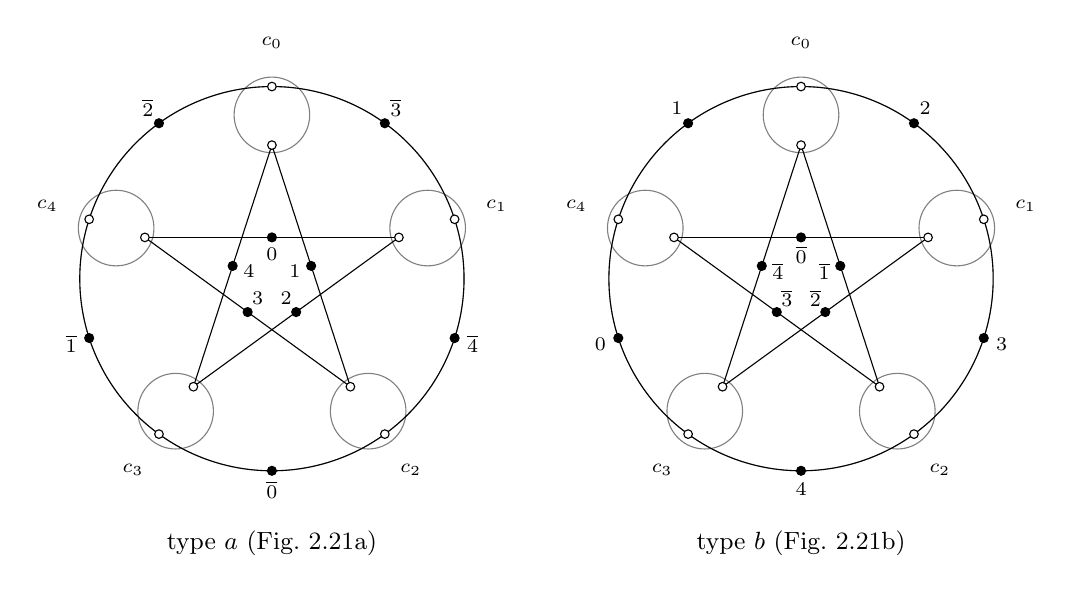
\begin{tikzpicture}[scale=0.8,
  hub/.style={circle,fill=black,inner sep=1.3pt},
  markdot/.style={circle,draw=black,fill=white,inner sep=1.1pt}]
\foreach \side/\xs in {0/0,1/8.4}{
 \begin{scope}[xshift=\xs cm]
  \draw[gray!60] (0,0) circle (3.05);
  \foreach \i in {0,...,4}{
    \pgfmathsetmacro{\ang}{90-72*\i}
    \coordinate (I\i) at (\ang:2.12);
    \draw[gray] (\ang:2.6) circle (0.6);
    \node[font=\scriptsize] at (\ang:3.75) {$c_{\i}$};
  }
  \foreach \k in {0,...,4}{
    \pgfmathtruncatemacro{\km}{mod(\k+4,5)}
    \pgfmathtruncatemacro{\kp}{mod(\k+1,5)}
    \draw (I\km) -- (I\kp);
    \ifnum\side=0
      \pgfmathsetmacro{\sa}{90-72*(\k+2)}
      \pgfmathsetmacro{\ea}{90-72*(\k+3)}
      \pgfmathsetmacro{\ma}{90-72*(\k+2.5)}
      \node[hub] at ($(I\km)!0.5!(I\kp)$) {};
      \node[font=\scriptsize] at ($(I\km)!0.5!(I\kp)+(\ma:0.27)$) {$\k$};
      \draw (\sa:3.05) arc[start angle=\sa, end angle=\ea, radius=3.05];
      \node[hub] at (\ma:3.05) {};
      \node[font=\scriptsize] at (\ma:3.35) {$\overline{\k}$};
    \else
      \pgfmathsetmacro{\sa}{90-72*(\k+3)}
      \pgfmathsetmacro{\ea}{90-72*(\k+4)}
      \pgfmathsetmacro{\ma}{90-72*(\k+3.5)}
      \pgfmathsetmacro{\na}{90-72*(\k+2.5)}
      \node[hub] at ($(I\km)!0.5!(I\kp)$) {};
      \node[font=\scriptsize] at ($(I\km)!0.5!(I\kp)+(\na:0.27)$) {$\overline{\k}$};
      \draw (\sa:3.05) arc[start angle=\sa, end angle=\ea, radius=3.05];
      \node[hub] at (\ma:3.05) {};
      \node[font=\scriptsize] at (\ma:3.35) {$\k$};
    \fi
  }
  \foreach \i in {0,...,4}{ \node[markdot] at ({90-72*\i}:3.05) {}; \node[markdot] at (I\i) {}; }
  \node[font=\small] at (0,-4.2) {\ifnum\side=0 type $a$ (Fig.~2.21a)\else type $b$ (Fig.~2.21b)\fi};
 \end{scope}}
\end{tikzpicture}
\caption{One block of each type (positions $c_0, \dots, c_4$ clockwise from the top). Open circles: the outer mark (on
the circle) and the inner mark (pentagram corner) of one row $t$ in each copy. Black dots: the hubs $(t,k)$, labelled
$k$, and $(t,\bk k)$, labelled $\bar k$. Each hub is adjacent to the two marks at the ends of its edge or arc.}
\label{fig:blocks}
\end{figure}

The figures do not say which colour class the inner dot is. In Figs.~2.3, 2.6 and 2.18 the class above the dashed line
is class $j = 0$, and in both Figs.~2.21 the outer dot of the top copy is above the dashed line. With class $0$ = points
this gives \textbf{reading 1}: outer = points and inner = lines in every copy. \textbf{Reading 2} (used in the first
computations): unbarred $K_1$-vertices always on points and barred ones always on lines. The thesis does not say which
blocks are of type (a) and which of type (b) (``utilizando cualquiera de las dos estructuras''), so we allow any pattern.
Below we allow the inner class to be chosen freely in every copy; this contains both readings and their duals.

\subsection{Definition with exact neighbourhoods}

\begin{definition}[$\Om H_q$]\label{def:omega}
The data are a prime power $q$ and $\alpha = \lfloor (q+3)/2 \rfloor$; a block pattern
$(\tau_0, \dots, \tau_{\alpha-1}) \in \{a,b\}^\alpha$; an inner class $\iota(c) \in \{\pP, \lL\}$ for every copy $c$; and a
\emph{labelling}: bijections $P_c\colon \mathbb{Z}/N\mathbb{Z} \to \pP$ and $L_c\colon \mathbb{Z}/N\mathbb{Z} \to \lL$ for
every copy~$c$.
\begin{itemize}[leftmargin=1.5em]
\item \emph{Copies.} $c = 5B + i$ with block $B \in \{0, \dots, \alpha-1\}$ and position $i \in \mathbb{Z}_5$; $5\alpha$
  copies. Copy vertices $(c,x)$, $x \in \pP \cup \lL$, with $(c,x) \sim (c,y)$ when $x$ and $y$ are incident.
\item \emph{Hubs} (the copies of $K_1$). $(t,k)$ and $(t,\bk k)$ for $t \in \mathbb{Z}/N\mathbb{Z}$ (the \emph{row}) and
  $k \in \mathbb{Z}_5$. The hub \emph{classes} are $k = \{(t,k)\}_t$ (unbarred) and $\bk k = \{(t,\bk k)\}_t$ (barred).
\item \emph{Copies met by a class} (positions mod $5$):
  \begin{align*}
  C(k) &= \{5B + k - 1,\ 5B + k + 1 : \tau_B = a\} \cup \{5B + k + 3,\ 5B + k + 4 : \tau_B = b\},\\
  C(\bk k) &= \{5B + k + 2,\ 5B + k + 3 : \tau_B = a\} \cup \{5B + k - 1,\ 5B + k + 1 : \tau_B = b\}.
  \end{align*}
\item \emph{Where a class sits.} In a copy $c$ of a block of type $a$, unbarred classes sit on the inner class $\iota(c)$
  and barred classes on the outer class; in a block of type $b$, unbarred classes sit on the outer class and barred
  classes on the inner class.
\item \emph{Hub edges.} For $c \in C(Y)$: $(t,Y) \sim (c, P_c(t))$ if $Y$ sits on points in $c$, and
  $(t,Y) \sim (c, L_c(t))$ if $Y$ sits on lines in~$c$.
\end{itemize}
The \textbf{thesis labelling} is $P_c = P_0$, $L_c = L_0$ for all $c$. \textbf{Reading 1}: $\iota(c) = \lL$ for all $c$.
\textbf{Reading 2}: $\iota(c) = \pP$ in $a$-blocks and $\lL$ in $b$-blocks (then unbarred hubs sit on points everywhere).
Gómez's $\Om H_q$ is the thesis labelling with any pattern and either reading.
\end{definition}

\emph{Exact neighbourhoods.} Write $m_c(t)$ for the inner mark of row $t$ in copy $c$ ($P_c(t)$ if $\iota(c) = \pP$,
$L_c(t)$ if $\iota(c) = \lL$) and $\bar m_c(t)$ for the outer mark. For $c = 5B + i$:
\begin{center}\small
\begin{tabular}{@{}lp{11.2cm}@{}}
\toprule
vertex & neighbours\\
\midrule
$(c,x)$ & $(c,y)$ for the $q+1$ elements $y$ incident with $x$, and two hubs:\\
\quad $\tau_B = a$, $x = m_c(t)$ & $(t, i-1)$, $(t, i+1)$\\
\quad $\tau_B = a$, $x = \bar m_c(t)$ & $(t, \bk{i+2})$, $(t, \bk{i+3})$\\
\quad $\tau_B = b$, $x = m_c(t)$ & $(t, \bk{i-1})$, $(t, \bk{i+1})$\\
\quad $\tau_B = b$, $x = \bar m_c(t)$ & $(t, i+1)$, $(t, i+2)$\\
$(t,k)$ & $(c, m_c(t))$ for $c = 5B + k \pm 1$ in blocks with $\tau_B = a$;\newline
  $(c, \bar m_c(t))$ for $c = 5B+k+3,\ 5B+k+4$ in blocks with $\tau_B = b$\\
$(t,\bk k)$ & $(c, \bar m_c(t))$ for $c = 5B + k+2,\ 5B+k+3$ in blocks with $\tau_B = a$;\newline
  $(c, m_c(t))$ for $c = 5B+k\pm1$ in blocks with $\tau_B = b$\\
\bottomrule
\end{tabular}
\end{center}

\begin{lemma}[Theorem; parameters]\label{lem:params}
For every pattern, inner classes and labelling, $\Om H_q$ is a simple bipartite graph on $10(\alpha+1)N = 5(\alpha+1)N_1$
vertices, with $5\alpha N(q+1) + 20\alpha N$ edges; copy vertices have degree $q+3$ and hubs degree $2\alpha$, so
$\Delta = q + 3 = \Delta_1 + 2$. Every hub meets $2\alpha$ of the $5\alpha$ copies and misses $3\alpha$.
\end{lemma}

\begin{proof}
The copy at position $i$ of an $a$-block is met by the unbarred classes $i \pm 1$ and the barred classes $i+2, i+3$; of a
$b$-block, by the unbarred classes $i+1, i+2$ and the barred classes $i \pm 1$. So each copy is met by exactly two
classes of each bar, the two classes of one bar sit on the same type, and each class has one hub per row. Every element
of a copy is the mark of exactly one row of its type, so it gets exactly two hubs. A class meets two distinct copies in
each block. For the colouring, give unbarred hubs colour $0$; in every copy, the type on which the unbarred classes sit
colour $1$ and the other type colour $0$; barred hubs colour $1$. Copy edges join a point and a line, so every edge has
ends of different colours.
\end{proof}

\section{Theorem 1: one label (also in Lean)}\label{sec:one}

\begin{theorem}[projection]\label{thm:one}
Let $B$ be a graph and $G$ a graph whose vertices are of two kinds: \emph{copy vertices} $v$, each with a copy index
$c(v) \in J$ and a label $f(v) \in V(B)$, and \emph{new vertices} $x$, each with a label $f(x) \in V(B)$. Assume
\begin{enumerate}[label=(h\arabic*)]
\item if $u \sim w$ are copy vertices, then $c(u) = c(w)$ and $f(u) \sim f(w)$ in $B$;
\item every neighbour $w$ of a new vertex $x$ is a copy vertex with $f(w) = f(x)$;
\item no two new vertices are adjacent.
\end{enumerate}
If $x$ is a new vertex with no neighbour in copy $j$, and $v$ is a copy vertex with $c(v) = j$, then
$d_G(x,v) \ge d_B(f(x), f(v)) + 3$.
\end{theorem}

\begin{proof}
Let $(x = w_0, w_1, \dots, w_\ell = v)$ be a walk. By (h2), $w_1$ is a copy vertex with $f(w_1) = f(x)$. Let $m$ be the
number of new vertices among $w_1, \dots, w_{\ell-1}$. A new vertex $w_i$ ($0 < i < \ell$) has copy vertices $w_{i-1}$,
$w_{i+1}$ on both sides (h2, h3), with $f(w_{i-1}) = f(w_i) = f(w_{i+1})$; every other edge $w_iw_{i+1}$ ($i \ge 1$)
joins two copy vertices and maps to an edge of $B$ by (h1). Deleting the $m$ new vertices and one of the two equal labels
around each, the labels of $w_1, \dots, w_\ell$ form a walk in $B$ from $f(x)$ to $f(v)$ of length $\ell - 1 - 2m$. So
$\ell \ge d_B(f(x), f(v)) + 1 + 2m$. If $m = 0$, then $w_1, \dots, w_\ell$ are copy vertices joined by copy edges, so by
(h1) $c(w_1) = c(v) = j$ and $w_1$ is a neighbour of $x$ in copy $j$, a contradiction. So $m \ge 1$.
\end{proof}

\noindent\textbf{Lean.} \file{BipartiteDD.LeanMaxx.Projection.edist_ge} in
\file{lean/BipartiteDD/LeanMaxx/Projection/Main.lean} (walk lemmas in \file{Walk.lean}). Copies are encoded by
\texttt{c : V → Option ι} (\texttt{none} = new vertex) and labels by \texttt{f : V → β}:
\begin{Verbatim}[fontsize=\small,frame=single,framesep=2mm]
theorem edist_ge
    (h1 : ∀ u w i j, G.Adj u w → c u = some i → c w = some j → i = j ∧ B.Adj (f u) (f w))
    (h2 : ∀ x w, G.Adj x w → c x = none → c w ≠ none ∧ f w = f x)
    (h3 : ∀ x w, G.Adj x w → c x = none → c w = none → False)
    {x v : V} (hx : c x = none) {j : ι} (hmiss : ∀ w, G.Adj x w → c w ≠ some j)
    (hv : c v = some j) :
    (B.dist (f x) (f v) + 3 : ℕ∞) ≤ G.edist x v
\end{Verbatim}
The corollary \file{ediam_ge} gives \texttt{(D₁ + 3 : ℕ∞) ≤ G.ediam} when \texttt{B.edist t s = D₁},
\texttt{f x = t}, \texttt{f v = s}. \texttt{\#print axioms} gives only \texttt{propext}, \file{Classical.choice},
\file{Quot.sound}. An independent session rebuilt the modules (Lean v4.34.1, Mathlib as pinned), regenerated the
axioms output byte for byte, searched the files for \texttt{sorry}, \texttt{admit}, \file{native_decide} and
similar, and read the statement against the specification (\file{research/lean-maxx/VERIFY.md}). The Lean statement is
slightly more general than Theorem~\ref{thm:one} ($B$ need not be bipartite and copies need not be whole copies;
\file{B.dist} is $0$ when \texttt{f x} and \texttt{f v} are not connected, which only weakens it). That $\Om H_q$
satisfies (h1)--(h3) is checked in Corollary~\ref{cor:one}; it is not part of the Lean files.

\begin{corollary}[Theorem]\label{cor:one}
Take the thesis labelling and inner classes for which every hub class sits on one type in all copies it meets (reading 2;
its dual; reading 1 when all blocks have one type). Then for every $q$, every pattern and every pairing $\sigma$: for
every hub $x$ and every copy $j$ that $x$ misses, the $q^5$ vertices $(j,y)$ with $y$ opposite the mark of $x$ are at
distance $\ge 9$ from $x$. So $\operatorname{diam} \Om H_q \ge 9$. More generally, for any bipartite graph $B_1$ with two
vertices at distance $D_1$, $\Om B_1$ in reading 2 has diameter $\ge D_1 + 3$.
\end{corollary}

\begin{proof}
Put $c((c,y)) = c$ and $f((c,y)) = y$, and label a hub by its mark ($P_0(t)$ or $L_0(t)$, the same in all copies by
assumption). Copy edges satisfy (h1), hub edges (h2) by Definition~\ref{def:omega}, and there are no hub--hub edges. Every
hub misses $3\alpha \ge 1$ copies (Lemma~\ref{lem:params}), and every vertex of $I$ has $q^5$ opposite vertices
(Lemma~\ref{lem:profile}). Apply Theorem~\ref{thm:one}. For general $B_1$: in reading 2 the unbarred classes sit on all
labels of class $0$ and the barred classes on all labels of class $1$, so whichever class holds the pair, some hub
carries one of its labels.
\end{proof}

For instance, if $P_0(t) = e_0$, the hub $(t,k)$ (reading 2) is at distance $\ge 9$ from every point
$\langle(x_3^2 - x_1x_5 - x_2x_6, x_1, x_2, x_3, 1, x_5, x_6)\rangle$ of each of the $3\alpha$ copies it misses
(Example in \S\ref{sec:hexagon}).

\begin{computer}[the hexagons]\label{cc:hex}
The incidence graphs of $H(q)$ used in the computations were checked by all-pairs BFS (no symmetry assumed): $2N$
vertices, bipartite, $(q+1)$-regular, diameter $6$, girth $12$. Three times: \file{hexq6.c} (this model) with
\file{apsp_mt}, $q = 3,4,5,7,8,9,11,13$; \file{hexgen.c}, \file{hexgf.c} (split octonions) with
\file{bitapsp.c}, $q = 2,3,4,5,7,8,9,11,13$; \file{buildhex.py} (split octonions) with \file{ghcheck.c},
$q = 3,7,8,9$. A $(q+1)$-regular bipartite graph on $2N$ vertices with diameter $6$ and girth $12$ is the incidence graph
of a generalized hexagon of order~$(q,q)$.
\end{computer}

\begin{computer}[the thesis graphs]\label{cc:thesis}
\begin{enumerate}[label=(\alph*),leftmargin=1.5em]
\item \emph{Exact diameters} (both block types present). $\Om H_3$ and $\Om H_5$ ($195{,}300$ vertices, the thesis's
  $(8,8)$ value): $9$ by all-pairs BFS in both readings, $\sigma$ the identity and two random $\sigma$, patterns $aba$,
  $aab$, $abab$, $aabb$ (twice). $\Om H_7$: $9$ in reading 2 ($ababa$) and reading 1 ($ababa$, random $\sigma$), by BFS
  from $117{,}648$ sources, one in every orbit of the rotation and the block swaps, each automorphism checked edge by
  edge. $\Om H_9$: $9$ in reading 2 ($aaabbb$; $18$ orbits of a group generated by the rotation, block swaps, a Singer
  cycle and a transvection of $H(9)$, all checked on the $27{,}900{,}600$ edges) and in reading 1 (Singer-equivariant
  $\sigma$, $4{,}380$ orbits); again $9$ in reading 2 and in reading 1 with a random $\sigma$ from $398{,}580$ orbit
  representatives (second program).
\item \emph{All six thesis values.} BFS from a hub gives eccentricity $9$ for $\Om H_5$, $\Om H_7$, $\Om H_8$, $\Om H_9$,
  $\Om H_{11}$, $\Om H_{13}$ at the thesis orders, in both readings (twice; a third program for reading 1). In reading 2
  the vertices at distance $9$ from a hub $(t,k)$ are exactly the points opposite $t$ in the $3\alpha$ copies it misses:
  $3\alpha q^5$ = $252{,}105$ ($q = 7$), $491{,}520$ ($8$), $1{,}062{,}882$ ($9$), $3{,}382{,}071$ ($11$),
  $8{,}911{,}032$ ($13$).
\item \emph{One block type}: diameter $10$ (all pairs at $q = 2, 3, 5$; orbit BFS at $q = 7, 9$).
\item Explicit pairs at distance $9$ for every cell: \file{checks/witness_omega_thesis.txt} (table audit),
  \file{research/d12D8/omega/witness_pairs.txt} (own-12-8).
\end{enumerate}
\end{computer}

\section{Theorem 2: two labels}\label{sec:two}

In reading 1 with both block types, an unbarred hub $(t,k)$ sits on line $L_0(t)$ in $a$-blocks and on point $P_0(t)$ in
$b$-blocks, so Theorem~\ref{thm:one} does not apply. The following count covers every reading.

\begin{theorem}\label{thm:two}
Let $q \ge 7$. Take $\Om H_q$ with the thesis labelling, any block pattern and any inner classes (so both readings and
every pairing $\sigma$). Let $x$ be a hub and $j$ a copy that $x$ misses. Then at least
\[
q^5 - (A + B + 1) = q^5 - 5q^4 - 8q^3 - 12q^2 - 16q - 10 > 0
\]
vertices of copy $j$ are at distance $\ge 9$ from $x$, where (sums over integers $e_i \ge 0$)
\[
A = \sum_{e_1 + e_2 \in \{0,2,4\}} s_{e_1}s_{e_2} = 5q^4 + 8q^3 + 6q^2 + 4q + 2, \qquad
B = \sum_{e_1+e_2+e_3 \le 2} s_{e_1}s_{e_2}s_{e_3} = 6q^2 + 12q + 7 .
\]
In particular $\operatorname{diam} \Om H_q \ge 9$.
\end{theorem}

\begin{center}\small
\begin{tabular}{@{}rrrrrr@{}}
\toprule
$q$ & $A$ & $B$ & $A + B + 1$ & $q^5$ & far vertices per missed copy ($\ge$)\\
\midrule
7 & 15,073 & 385 & 15,459 & 16,807 & 1,348\\
8 & 24,994 & 487 & 25,482 & 32,768 & 7,286\\
9 & 39,161 & 601 & 39,763 & 59,049 & 19,286\\
11 & 84,625 & 865 & 85,491 & 161,051 & 75,560\\
13 & 161,449 & 1,177 & 162,627 & 371,293 & 208,666\\
\bottomrule
\end{tabular}
\end{center}

\begin{proof}
Let $\tau$ be the involution of $\pP \cup \lL$ with $\tau(P_0(s)) = L_0(s)$ for every row $s$. Every hub of row $s$ is
adjacent, in each copy it meets, to $P_0(s)$ or to $L_0(s)$. Let $x$ have row $t$. By Lemma~\ref{lem:params}, in copy $j$
one type $T \in \{\pP, \lL\}$ has the colour of the neighbours of $x$; let $z = P_0(t)$ if $T = \pP$ and $z = L_0(t)$ if
$T = \lL$. We show that at most $A + B + 1$ elements $w \in \opp(z)$ have $d(x,(j,w)) \le 8$; as $|\opp(z)| = q^5$, the
others are at distance $\ge 9$.

Let $w \in \opp(z)$; it has type $T$. The graph is bipartite and $(j,w)$ has the colour of the neighbours of $x$, so
$d(x,(j,w))$ is odd; suppose it is $\le 7$ and take a shortest path. It leaves $x$ to a vertex $(c_1, a_0)$ with
$a_0 \in \{z, \tau(z)\}$, then alternates walks inside copies with passes copy $\to$ hub $\to$ copy. A pass through a hub
of row $s$ goes from $(c, a)$ to $(c', a')$ with $a, a' \in \{P_0(s), L_0(s)\}$, so $a' = a$ (a \emph{stay}) or
$a' = \tau(a)$ (a \emph{switch}). Since $x$ misses $j$ there is at least one pass. With $e$ copy edges and $p \ge 1$
passes the length is $1 + e + 2p \le 7$ and odd, so $e$ is even, $e \le 4$ and $p \le 3 - e/2$. Let $r \le p$ be the
number of switches. Merging the stays, the labels form a walk in $I$ from $a_0$ with $e$ edges in total, with $\tau$
applied $r$ times in between, ending at $w$. Every edge of $I$ and every switch changes the type, and $w$ has the type of
$z$, so $r$ is even if $a_0 = z$ and odd if $a_0 = \tau(z)$. The set of ends of walks of length $f$ from a vertex $u$ is
$\bigcup S_g(u)$ over $g \le f$, $g \equiv f \pmod 2$, of size at most the sum of the $s_g$. So:
\begin{itemize}[leftmargin=1.5em]
\item $a_0 = z$, $r = 0$: $w$ ends a walk of length $e \le 4$ from $z$, so $d(z,w) \le 4$ and $w \notin \opp(z)$.
\item $a_0 = z$, $r = 2$: $p \ge 2$, so $e \le 2$; the label walk is $z \to (f_1$ edges$) \to u_1$, switch,
  $\to (f_2) \to u_2$, switch, $\to (f_3) \to w$, with $f_1 + f_2 + f_3 = e \le 2$. At most $B$ such $w$.
\item $a_0 = \tau(z)$, $r = 1$: $\tau(z) \to (f_1) \to u_1$, switch, $\to (f_2) \to w$ with $f_1 + f_2 = e \in \{0,2,4\}$.
  At most $A$ such $w$.
\item $a_0 = \tau(z)$, $r = 3$: $p = 3$, $e = 0$, and $w = \tau^4(z) = z \notin \opp(z)$ (counted as $1$ to match the
  earlier reports).
\end{itemize}
The closed forms are expansions (for $A$: $s_0s_0 + 2s_0s_2 + s_1s_1 + 2s_0s_4 + 2s_1s_3 + s_2s_2$). Finally, for
$q \ge 7$, $q^4(q-5) \ge 2q^4 \ge 14q^3$, so
$q^5 - 5q^4 - 8q^3 - 12q^2 - 16q - 10 \ge 6q^3 - 12q^2 - 16q - 10 \ge 30q^2 - 16q - 10 > 0$.
\end{proof}

\begin{remark}
The proof uses only: the graph is bipartite; all copies carry the labels $P_0, L_0$; every hub of row $s$ is adjacent, in
each copy it meets, only to $P_0(s)$ or $L_0(s)$; there are no hub--hub edges; $x$ misses a copy. It does not use that $x$
meets both types, so it also covers the hubs to which Theorem~\ref{thm:one} applies. (This applies the two corrections
asked for by the referee of the first write-up: ``bipartite'' belongs in the hypothesis, and the appeal to
Theorem~\ref{thm:one} for single-label hubs is not needed.) For $q \le 6$ the count is not enough ($A + B + 1 > q^5$); see
\ref{cc:small}.
\end{remark}

\begin{corollary}[Theorem]\label{cor:two}
As defined in the thesis (every copy carries the same labels, and a copy of $K_1$ with label $t$ is joined only to
vertices labelled $t$), $\Om H_q$ has diameter $\ge 9$ for $q = 7, 8, 9, 11, 13$, under every reading of Figs.~2.21a/b,
every pattern of block types and every pairing of point labels with line labels. These are the six table entries.
\end{corollary}

\begin{computer}[$q = 3, 5$]\label{cc:small}
Where the count of Theorem~\ref{thm:two} fails, all-pairs BFS gives diameter $9$ for $\Om H_3$ and $\Om H_5$ in both
readings and for several $\sigma$ (\ref{cc:thesis}(a)). Under reading 1 ($\sigma$ the identity or random), the largest
number of opposite vertices of the right type within distance $7$ of a hub, in a copy it misses, was $7{,}562$--$8{,}039$
at $q = 7$ (bound $15{,}459$), $13{,}950$ at $q = 8$ ($25{,}482$), $22{,}771$--$22{,}825$ at $q = 9$ ($39{,}763$),
$52{,}372$ at $q = 11$ ($85{,}491$) and $104{,}225$ at $q = 13$ ($162{,}627$).
\end{computer}

\section{Relabelling the copies}\label{sec:relabel}

Diameter $\ge 9$ comes from the shared labels. A labelling that differs from copy to copy is not in the thesis
(\S\S2.7--2.9 use one labelling for all copies), but it is the obvious repair, and at $q = 2, 3$ it works
(\ref{cc:q23}). This section shows that it cannot work at the table's $q$ with labellings that respect the geometry.

\subsection{The model}
A labelling $(P_c, L_c)$ as in Definition~\ref{def:omega} gives each copy one point labelling and one line labelling,
used by every hub class of the corresponding type that meets the copy. For a hub class $Y$ and copies $c, d \in C(Y)$,
the \textbf{transfer} $T_Y(c \to d)$ maps the mark of row $t$ in $c$ to the mark of row $t$ in $d$: it is
$P_dP_c^{-1}$, $L_dL_c^{-1}$, $L_dP_c^{-1}$ or $P_dL_c^{-1}$, according to the types $Y$ sits on in $c$ and $d$.

\begin{definition}\label{def:geo}
A labelling is \textbf{geometric} if every transfer is the restriction (to $\pP$ or to $\lL$) of an automorphism of $I$:
a collineation of $H(q)$ or, when $q$ is a power of $3$, a duality.
\end{definition}

Labellings chosen per pair (class, copy), in which the two classes of one bar meeting a copy may use different
bijections, are outside this model even when every transfer is a collineation; see \S\ref{sec:open}.

\begin{lemma}[Theorem; one automorphism per copy]\label{lem:oneaut}
Relabelling every copy $c$ of a graph $\Om H_q$ by an automorphism $g_c$ of $I$ (replacing every vertex $(c,y)$ by
$(c, g_c(y))$) gives an isomorphic graph. Applied to the thesis graph: for collineations $g_c$ this is the labelling
$P_c = g_cP_0$, $L_c = g_cL_0$; for dualities, the labelling $P_c = g_cL_0$, $L_c = g_cP_0$ with the inner class of $c$
exchanged. Such a graph is isomorphic to the thesis graph it came from, so its diameter is $\ge 9$ by
Corollary~\ref{cor:one} (if that graph is in reading 2: every $q$) and by Corollary~\ref{cor:two} (every reading,
$q \ge 7$).
\end{lemma}

\begin{proof}
Copy edges are preserved because $g_c$ is an automorphism of $I$; hub edges are carried along by definition.
\end{proof}

\begin{lemma}[Theorem; reduction and normal form]\label{lem:reduce}
Take a geometric labelling, with any pattern and inner classes.
\begin{enumerate}[label=(\alph*)]
\item If $q$ is not a power of $3$, every hub class sits on one type in all copies it meets, all unbarred classes sit
  on the same type and all barred classes on the other: the inner classes are those of reading 2 or of its dual.
\item If $q$ is a power of $3$, the graph is isomorphic to one with a geometric labelling in reading 2 (same pattern).
\item In reading 2 and in its dual, the graph is isomorphic to one with $P_c = P_0$ for all $c$ and $L_c = \lambda_cL_0$
  with collineations $\lambda_c$ (the \emph{normal form}). We call the bar that sits on points the \textbf{point bar}
  $\cP$ (unbarred in reading 2, barred in its dual) and the other the \textbf{line bar} $\cL$.
\end{enumerate}
\end{lemma}

\begin{proof}
(a) A transfer from a copy where $Y$ sits on points to one where it sits on lines maps $\pP$ to $\lL$; an automorphism of
$I$ doing that is a duality, and there is none (Fact~\ref{fact:aut}). In every copy the two unbarred classes sit on the
same type. The copies are linked by unbarred classes: inside a block, the pairs $\{k \pm 1\}$ (type $a$) or
$\{k+3, k+4\}$ (type $b$), $k \in \mathbb{Z}_5$, form a $5$-cycle on the positions, and every class meets every block. So
all unbarred classes sit on one type, and the barred classes sit on the other type in every copy.
(b) Fix a duality $\delta$ and relabel by $\delta$ every copy in which the unbarred classes sit on lines
(Lemma~\ref{lem:oneaut}). The new transfers are the old ones composed with $\delta^{\pm1}$, so they are still
automorphisms of $I$, and now all unbarred classes sit on points.
(c) The transfers of the point bar are restrictions of collineations to $\pP$, and that bar links all copies (as in
(a); for the barred classes the pairs are $\{k+2, k+3\}$ and $\{k \pm 1\}$). Fixing a copy $c_0$, every
$P_cP_{c_0}^{-1}$ is a product of transfers, so $P_c = a_cP_{c_0}$ with a collineation $a_c$; likewise
$L_c = b_cL_{c_0}$. Relabel copy $c$ by $a_c^{-1}$ (Lemma~\ref{lem:oneaut}): $P_c$ becomes $P_{c_0}$ and $L_c$ becomes
$a_c^{-1}b_cL_{c_0}$. Unbarred rows and barred rows are different vertices, so renaming the rows of each bar separately
gives $P_c = P_0$ and $L_c = \lambda_cL_0$ with $\lambda_c = a_c^{-1}b_c$.
\end{proof}

From now on we use the normal form, identify the rows of the point bar with points through $P_0$ (so the hub $(t,X)$,
$X \in \cP$, is adjacent to the point $t$ of every copy in $C(X)$), and let the collineations $\lambda_c$ act on $\pP$
and on $\lL$.

\subsection{Routes reach balls}
For $X \in \cP$ and $c' \notin C(X)$ let $N(X,c')$ be the set of copies $c_1 \in C(X)$ such that some class of $\cL$
meets both $c_1$ and $c'$.

\begin{lemma}[Theorem; routes]\label{lem:routes}
Let $X \in \cP$, $c' \notin C(X)$ and $t \in \pP$. Every point $v$ of copy $c'$ with $d((t,X),(c',v)) \le 7$ lies in
\[
B(t,4) \ \cup \bigcup_{c_1 \in N(X,c')} B(\lambda_{c'}\lambda_{c_1}^{-1}(t), 4) \ \cup \bigcup_{(c,d) \in W_2}
B(\lambda_c\lambda_d^{-1}(t), 2),
\]
where $W_2$ is the set of ordered pairs of distinct copies of three kinds: $(c', c_2)$ with $c_2$ sharing a class of
$\cP$ with some $c_1 \in C(X)$ and a class of $\cL$ with $c'$; $(c', c_1)$ with $c_1 \in C(X)$ and some $c_2$ sharing a
class of $\cL$ with $c_1$ and one with $c'$; $(c_2, c_1)$ with $c_1 \in C(X)$ and $c_2$ sharing a class of $\cL$ with
$c_1$ and a class of $\cP$ with $c'$.
\end{lemma}

\begin{proof}
A path from $h = (t,X)$ to $(c',v)$ goes to the point $t$ of a copy $c_1 \in C(X)$, then alternates walks inside copies,
of lengths $a_1, \dots, a_r \ge 0$, with $r-1$ passes copy $\to$ hub $\to$ copy, ending in $c'$. A hub meets each copy at
most once, so consecutive copies differ; $c_1 \ne c'$, so $r \ge 2$. The length is $1 + \sum a_i + 2(r-1) \le 7$, so
$\sum a_i \le 8 - 2r$ and $r \le 4$. A pass through a $\cP$-hub happens at a point and keeps it ($\cP$-hubs sit on the
same point in every copy). A pass through an $\cL$-hub $(m,Y)$ happens at a line and goes from $\lambda_cL_0(m)$ in $c$ to
$\lambda_dL_0(m)$ in $d$: it applies $\lambda_d\lambda_c^{-1}$. Collineations preserve distances, so by induction the
end lies in $B(g(t), \sum a_i)$, where $g$ is the product of the maps applied. The walk starts and ends at points and an
$\cL$-pass happens at a line, so the segments next to $\cL$-passes are odd and $\sum a_i$ is even.
\begin{itemize}[leftmargin=1.5em]
\item $r = 2$ ($\sum a_i \le 4$): a $\cP$-pass gives $g = \mathrm{id}$; an $\cL$-pass needs a class of $\cL$ meeting
  $c_1$ and $c'$, that is $c_1 \in N(X,c')$, and gives $g = \lambda_{c'}\lambda_{c_1}^{-1}$.
\item $r = 3$ ($\sum a_i \le 2$): $\cP$ then $\cP$ gives $\mathrm{id}$. $\cP$ then $\cL$ forces $a_1 = 0$,
  $a_2 = a_3 = 1$ and $g = \lambda_{c'}\lambda_{c_2}^{-1}$ (first kind). $\cL$ then $\cP$ forces $a_1 = a_2 = 1$,
  $a_3 = 0$ and $g = \lambda_{c_2}\lambda_{c_1}^{-1}$ (third kind). $\cL$ then $\cL$ forces $a_1 = a_3 = 1$, $a_2 = 0$:
  both passes use the same row $m$, so $g = \lambda_{c'}\lambda_{c_2}^{-1}\lambda_{c_2}\lambda_{c_1}^{-1} =
  \lambda_{c'}\lambda_{c_1}^{-1}$ (second kind).
\item $r = 4$: all $a_i = 0$, so the walk never reaches a line, all passes are $\cP$-passes, and $v = t$.\qedhere
\end{itemize}
\end{proof}

For a pair $(X, c')$ let $r_4 = |N(X,c')|$, and let $m_2$ be the number of pairs in $W_2$ that are not of the form
$(c', c_1)$ with $c_1 \in N(X,c')$. Different pairs may give the same map; counting pairs only overestimates.

\begin{corollary}[Theorem]\label{cor:count}
Every hub $(t,X)$ has at least $q^5 - r_4q^4 - m_2q^2$ points of $c'$ at distance $\ge 9$. If $r_4 = \alpha$, then
$m_2 \le (4\alpha - 1) + 2\alpha \cdot 2(2\alpha - 1) = 8\alpha^2 - 1$.
\end{corollary}

\begin{proof}
By Lemma~\ref{lem:balls}, $B(t,4)$ misses $\opp(t)$, each other radius-$4$ ball meets it in at most $q^4$ points and
each radius-$2$ ball in at most $q^2$. The remaining points of $\opp(t)$ in $c'$ are at distance $> 7$ from $(t,X)$, and
at odd distance, since all points of all copies have one colour; so at distance $\ge 9$. For the bound on $m_2$: the
first two kinds are pairs $(c', b)$ with $b \ne c'$, at most $5\alpha - 1 - r_4 = 4\alpha - 1$ of them outside the
radius-$4$ words; the third kind has $\le 2\alpha$ choices of $c_1$ and, since $c_1$ is met by two classes of $\cL$ that
meet $2\alpha$ copies each, $\le 2(2\alpha - 1)$ choices of $c_2$.
\end{proof}

\subsection{Starved pairs}
Call $(X, c')$ with $X \in \cP$, $c' \notin C(X)$ \textbf{starved} if $r_4 = \alpha$: exactly one copy of $C(X)$ per
block shares a class of $\cL$ with $c'$.

\begin{lemma}[Theorem]\label{lem:starved}
For every block pattern there are starved pairs with $X$ unbarred and starved pairs with $X$ barred:
\begin{itemize}[leftmargin=1.5em]
\item $X = k$ unbarred: $c' = 5B' + k + 3$ for a block $B'$ of type $a$; if all blocks are of type $b$, $c' = 5B' + k$.
\item $X = \bk k$ barred: $c' = 5B' + k + 3$ for a block $B'$ of type $b$; if all blocks are of type $a$,
  $c' = 5B' + k + 1$.
\end{itemize}
\end{lemma}

\begin{proof}
The classes meeting the copy at position $i$ are: in an $a$-block, unbarred $i \pm 1$ and barred $i+2, i+3$; in a
$b$-block, unbarred $i+1, i+2$ and barred $i \pm 1$.
For $X = k$ ($\cL$ = barred): $c'$ at position $k+3$ of an $a$-block has barred classes $\{k, k+1\}$. In an $a$-block,
$C(k)$ has positions $k-1$ (barred $\{k+1, k+2\}$: shares) and $k+1$ (barred $\{k+3, k+4\}$: does not); in a $b$-block,
positions $k+3$ (barred $\{k+2, k+4\}$: no) and $k+4$ (barred $\{k, k+3\}$: shares). If all blocks are of type $b$, $c'$
at position $k$ has barred $\{k-1, k+1\}$, and $C(k)$ has $k+3$ (barred $\{k+2, k+4\}$: shares $k + 4 = k - 1$) and $k+4$
(barred $\{k, k+3\}$: no).
For $X = \bk k$ ($\cL$ = unbarred): $c'$ at position $k+3$ of a $b$-block has unbarred $\{k+4, k\}$. In an $a$-block,
$C(\bk k)$ has $k+2$ (unbarred $\{k+1, k+3\}$: no) and $k+3$ (unbarred $\{k+2, k+4\}$: shares); in a $b$-block, $k-1$
(unbarred $\{k, k+1\}$: shares) and $k+1$ (unbarred $\{k+2, k+3\}$: no). If all blocks are of type $a$, $c'$ at position
$k+1$ has unbarred $\{k, k+2\}$, and $C(\bk k)$ has $k+2$ (unbarred $\{k+1, k+3\}$: no) and $k+3$ (unbarred
$\{k+2, k+4\}$: shares). In each case $c' \notin C(X)$.
\end{proof}

\begin{computer}[route words]\label{cc:routes}
For $\alpha = 5, 6, 7, 8$ and every block pattern (by block swaps only the number of $a$-blocks matters), the routes of
Lemma~\ref{lem:routes} were enumerated for every pair $(X, c')$:
\begin{itemize}[leftmargin=1.5em]
\item every pair has $r_4 \ge \alpha$, and no route ends in a radius-$0$ ball other than the identity;
\item for $\alpha = 5$ ($q = 7, 8$), every starved pair, of either bar and in every pattern, has $m_2 \le 140$;
\item for $\alpha = 6$ ($q = 9$), every starved pair has $m_2 \le 201$;
\item the best starved pair of the worst pattern has $m_2 = 134$ ($\alpha = 5$, patterns $aabbb$, $aaabb$), $197$
  ($\alpha = 6$, $aaabbb$), $262$ ($\alpha = 7$, $aaabbbb$), $347$ ($\alpha = 8$, $aaaabbbb$).
\end{itemize}
The last item twice (\file{routecount.c}, \file{routecount2.c} of the relabelling note; \file{myroutes.py},
\file{sweep.py} of its referee, which enumerates walks symbolically without using Lemma~\ref{lem:routes}'s
families). All four items were re-run for this note with the referee's enumerator for $\alpha = 5, 6, 7, 8$
(\file{starved.py}; the largest $m_2$ of a starved pair is $140$, $201$, $272$, $353$).
\end{computer}

\subsection{$q \ge 8$}

\begin{theorem}[computer-assisted for $q = 8, 9$]\label{thm:geo8}
Let $q \ge 8$. For every block pattern, every choice of inner classes (both readings, their duals, or any choice per
copy) and every geometric labelling, $\Om H_q$ has diameter $\ge 9$. More precisely, in the normal form, for every
starved pair $(X, c')$ every hub $(t,X)$ has at least $q^5 - \alpha q^4 - m_2q^2 > 0$ vertices of $c'$ at distance
$\ge 9$.
\end{theorem}

\begin{proof}
By Lemma~\ref{lem:reduce} we may assume the normal form, in reading 2 or its dual. Take a starved pair of the point bar
(Lemma~\ref{lem:starved}) and apply Corollary~\ref{cor:count}. For $q \ge 10$, $m_2 \le 8\alpha^2 - 1$ and the bound is
positive when $q^2(q - \alpha) \ge 8\alpha^2$; with $\alpha \le (q+3)/2$ it suffices that $q^2(q-3) \ge 4(q+3)^2$, that is
$q^3 - 7q^2 - 24q - 36 \ge 0$, which holds at $q = 10$ (value $24$) and beyond (the derivative $3q^2 - 14q - 24$ is
positive). For $q = 8$ ($\alpha = 5$), \ref{cc:routes} gives $m_2 \le 140$ and the bound is
$\ge 32{,}768 - 20{,}480 - 8{,}960 = 3{,}328$; for $q = 9$ ($\alpha = 6$), $m_2 \le 201$ and the bound is
$\ge 59{,}049 - 39{,}366 - 16{,}281 = 3{,}402$.
\end{proof}

\begin{center}\small
\begin{tabular}{@{}rrll@{}}
\toprule
$q$ & $\alpha$ & far vertices per hub of a starved class & best pair, worst pattern (\ref{cc:routes})\\
\midrule
8 & 5 & $\ge 3{,}328$ for every starved pair (uses \ref{cc:routes}) & 3,712\\
9 & 6 & $\ge 3{,}402$ for every starved pair (uses \ref{cc:routes}) & 3,726\\
11 & 7 & $\ge 11{,}253$ (by hand, $m_2 \le 391$) & 26,862\\
13 & 8 & $\ge 56{,}446$ (by hand, $m_2 \le 511$) & 84,162\\
\bottomrule
\end{tabular}
\end{center}

This covers $(11,8)$, $(12,8)$, $(14,8)$, $(15,8)$, $(16,8)$. Different starved pairs give disjoint sets of (hub, vertex)
pairs; summing, every geometric labelling leaves at least $3.33 \cdot 10^9$ far pairs at $q = 8$ and $7.43 \cdot 10^9$ at
$q = 9$ (Computer-checked twice: the relabelling note and its referee). The relabelling note first treated the other
readings separately for $q = 8, 9, 11, 13, 27$; its referee observed that Lemma~\ref{lem:reduce}(b) reduces them to
reading 2 for every $q$, which is how they are handled here.

\subsection{$q = 7$}
At $q = 7$ the bound of Corollary~\ref{cor:count} is negative ($16{,}807 - 5 \cdot 2{,}401 - 140 \cdot 49 = -2{,}058$),
so the overlaps of the five radius-$4$ balls must be used. Here $q$ is odd and $b$ is nondegenerate; $7$ is prime and not
a power of $3$, so the collineations are elements of $\GG(7) \le \mathrm{SO}(7,7)$ (Fact~\ref{fact:aut}) and the reading
is reading 2 or its dual (Lemma~\ref{lem:reduce}(a)). Fix a starved pair $(X, c')$ of the point bar and write
$g_1, \dots, g_5$ for the elements $\lambda_{c'}\lambda_{c_i}^{-1}$, $c_i \in N(X,c')$, and $y_i = g_i(t)$. By
Lemma~\ref{lem:perp}, $B(y,4) \cap \pP = y^\perp \cap Q(6,q)$ for a point $y$, so with $C_i := y_i^\perp \cap \opp(t)$
the points of $c'$ opposite $t$ within distance $7$ of $(t,X)$ lie in $C_1 \cup \dots \cup C_5$ and in at most
$m_2 \le 140$ balls of radius $2$.

\begin{lemma}[Theorem; overlaps, $q$ odd]\label{lem:overlap}
Let $y, y', t$ be distinct points of $Q(6,q)$.
\begin{enumerate}[label=(\alph*)]
\item If $y \ip y'$ and $t$ lies on the line $yy'$, then $y^\perp \cap y'^\perp \cap \opp(t) = \emptyset$. Otherwise $t$ is
  not on the line $yy'$ and $|y^\perp \cap y'^\perp \cap \opp(t)| \ge q^3 - q$.
\item If $y, y', y''$ are points not on one line, $|y^\perp \cap y'^\perp \cap y''^\perp \cap Q(6,q)| \le (q+1)^2$.
\item If $y, y', y''$ lie on one totally singular line $\ell$ not through $t$, all pairwise and triple intersections of
  $y^\perp \cap \opp(t)$, $y'^\perp \cap \opp(t)$, $y''^\perp \cap \opp(t)$ equal $X_\ell := \ell^\perp \cap \opp(t)$, and
  $|X_\ell| \ge q^3 - q$.
\end{enumerate}
\end{lemma}

\begin{proof}
If $y \ip y'$ the line $yy'$ is totally singular, and if $t$ is on it, $y^\perp \cap y'^\perp = (yy')^\perp \subseteq
t^\perp$. If $y \not\ip y'$, the line $yy'$ meets $Q(6,q)$ only in $y, y'$, so $t$ is not on it. In the remaining cases
$y^\perp \cap y'^\perp$ is the perp of a line, of vector dimension $5$: a parabolic $Q(4,q)$ (if $y \not\ip y'$) or a
cone with vertex the line $yy'$ over a conic (if $y \ip y'$); both have $q^3 + q^2 + q + 1$ points. Those not opposite $t$
are the points of $\Pi^\perp$, $\Pi = \langle y, y', t\rangle$ a plane. For three independent singular vectors the Gram
matrix of $b$ on $\Pi$ has zero diagonal, so its rank is $3$, $2$ or $0$ (a symmetric matrix with zero diagonal and
rank $1$ would be $vv^{T}$ with all $v_i^2 = 0$). The radical of $\Pi^\perp$ is $\Pi \cap \Pi^\perp$, of dimension
$0$, $1$ or $3$. In the first case $\Pi^\perp$ (dimension $4$) carries a nondegenerate form with $(q+1)^2$ or $q^2+1$
singular points; in the second it is a cone over a conic, $q^2+q+1$ points; in the third $\Pi$ is totally singular and
$\Pi^\perp = \Pi \oplus \langle w\rangle$ with $\Q(w) \ne 0$ ($Q(6,q)$ has no totally singular subspace of vector
dimension $4$), so its singular points are those of $\Pi$, $q^2+q+1$. So $|\Pi^\perp \cap Q(6,q)| \le (q+1)^2$, which
gives (a) and, with $\Pi = \langle y, y', y''\rangle$, (b). (c): $y^\perp \cap y'^\perp = \ell^\perp \subseteq y''^\perp$,
and $|X_\ell| \ge q^3 - q$ by (a).
\end{proof}

\begin{lemma}[Theorem; coincidences; uses $m_2 \le 140$ from \ref{cc:routes}]\label{lem:coinc}
If two of $t, y_1, \dots, y_5$ coincide, the hub $(t,X)$ has at least
$q^5 - 4q^4 - 140q^2 = 16{,}807 - 9{,}604 - 6{,}860 = 343$ vertices of $c'$ at distance $\ge 9$.
\end{lemma}

\begin{proof}
At most four distinct centres other than $t$ remain; argue as in Corollary~\ref{cor:count}.
\end{proof}

Now let $t, y_1, \dots, y_5$ be distinct. Call $y_i, y_j$ \textbf{aligned} if they lie on one totally singular line
through $t$ (then $C_i \cap C_j = \emptyset$ by Lemma~\ref{lem:overlap}(a)); the aligned classes partition
$\{y_1, \dots, y_5\}$. A \textbf{rich line} is a maximal set of at least three $y_i$ on one line of $\PG(6,q)$ not
through $t$. Three collinear singular points span a totally singular line, so every collinear triple of $y$'s lies in an
aligned class or in a rich line; a rich line meets each aligned class at most once, and two rich lines share at most one
point.

\begin{lemma}[Theorem; the configuration types at $q = 7$]\label{lem:types}
Let $A$ be the number of aligned pairs, $T$ the number of triples meeting three different aligned classes, and
$R_3 = \sum \binom{m}{3}$ over the rich lines ($m$ points each). Then
\[
|C_1 \cup \dots \cup C_5| \le U := 5q^4 - (10 - A - R_3)(q^3 - q) + (T - R_3)(q+1)^2,
\]
except when one rich line holds all five points, where $U := 5q^4 - 4(q^3 - q)$. Up to relabelling there are exactly
$17$ configuration types; for $q = 7$ they are listed in Table~\ref{tab:types}, with
$F = 16{,}807 - U - 6{,}860$ and the number $p$ of pairs among $\{t, y_1, \dots, y_5\}$ that are perpendicular in every
configuration of the type, $p = \sum_{s \ge 2}\bigl(s + \binom{s}{2}\bigr)$ over aligned classes of size $s$ plus
$\sum \binom{m}{2}$ over rich lines. In the $9$ types with $F \le 0$, $p \ge 6$.
\end{lemma}

\begin{table}[ht]
\centering\small
\begin{tabular}{@{}llrrrrrr@{}}
\toprule
aligned classes & rich lines & $A$ & $T$ & $R_3$ & $U$ & $F$ & $p$\\
\midrule
5 & -- & 10 & 0 & 0 & 12,005 & $-2{,}058$ & 15\\
4, 1 & -- & 6 & 0 & 0 & 10,661 & $-714$ & 10\\
3, 2 & -- & 4 & 0 & 0 & 9,989 & $-42$ & 9\\
3, 1, 1 & -- & 3 & 3 & 0 & 9,845 & $102$ & 6\\
3, 1, 1 & 3 & 3 & 3 & 1 & 10,117 & $-170$ & 9\\
2, 2, 1 & -- & 2 & 4 & 0 & 9,573 & $374$ & 6\\
2, 2, 1 & 3 & 2 & 4 & 1 & 9,845 & $102$ & 9\\
2, 2, 1 & 3, 3 & 2 & 4 & 2 & 10,117 & $-170$ & 12\\
2, 1, 1, 1 & -- & 1 & 7 & 0 & 9,429 & $518$ & 3\\
2, 1, 1, 1 & 3 & 1 & 7 & 1 & 9,701 & $246$ & 6\\
2, 1, 1, 1 & 3, 3 & 1 & 7 & 2 & 9,973 & $-26$ & 9\\
2, 1, 1, 1 & 4 & 1 & 7 & 4 & 10,517 & $-570$ & 9\\
1, 1, 1, 1, 1 & -- & 0 & 10 & 0 & 9,285 & $662$ & 0\\
1, 1, 1, 1, 1 & 3 & 0 & 10 & 1 & 9,557 & $390$ & 3\\
1, 1, 1, 1, 1 & 3, 3 & 0 & 10 & 2 & 9,829 & $118$ & 6\\
1, 1, 1, 1, 1 & 4 & 0 & 10 & 4 & 10,373 & $-426$ & 6\\
1, 1, 1, 1, 1 & 5 & 0 & 10 & 10 & 10,661 & $-714$ & 10\\
\bottomrule
\end{tabular}
\caption{The $17$ configuration types of Lemma~\ref{lem:types} at $q = 7$ ($q^4 = 2{,}401$, $q^3 - q = 336$,
$(q+1)^2 = 64$, $140q^2 = 6{,}860$).}
\label{tab:types}
\end{table}

\begin{proof}
$|C_i| = q^4$ (Lemma~\ref{lem:balls}, $y_i \ne t$). By Bonferroni, $|\bigcup C_i| \le S_1 - S_2 + S_3$, with $S_k$ the
sum of the $k$-fold intersections. By Lemma~\ref{lem:overlap}: an aligned pair contributes $0$ to $S_2$, and every triple
containing one contributes $0$ to $S_3$; a pair or triple inside a rich line $\ell$ contributes $|X_\ell|$; every other
pair contributes $\ge q^3 - q$, and every other triple (it is not collinear) $\le (q+1)^2$. A rich line with
$m \in \{3,4\}$ points contributes $-(\binom m2 - \binom m3)|X_\ell| = -2|X_\ell| \le -2(q^3 - q)$. Collecting terms gives
$U$. If all five points lie on one rich line, all pairwise intersections equal $X_\ell$, so
$|\bigcup C_i| = 5q^4 - 4|X_\ell|$ exactly. The types: two $3$-subsets of a $5$-set that share at most one point share
exactly one, and a third $3$-subset would share two points with one of them; a $4$- or $5$-point rich line leaves no room
for another. So the systems of rich lines are: none, one $3$-line, two $3$-lines through a common point, one $4$-line,
one $5$-line. A rich line takes at most one point from each aligned class, which leaves exactly the $17$ rows (partitions
$5$, $41$, $32$: no rich line; $311$: none or one $3$-line; $221$: none, one, or two $3$-lines through the singleton;
$2111$: none, $3$, $3+3$, $4$; $11111$: none, $3$, $3+3$, $4$, $5$). The numbers $A$, $T$, $R_3$ and $p$ depend only on
the row.
\end{proof}

The table was also produced by three programs: \file{degen.py} of the relabelling note, \file{mytypes.py} of its
referee, and \file{types43.py}, written from scratch for this note. The referee also built $2{,}500$ explicit
configurations in $Q(6,7)$ and found no union above the bound of its type.

\begin{lemma}[Theorem; few points are moved to perpendicular points]\label{lem:perpbound}
Let $q$ be odd with $3 \mid q - 1$, and let $h \in \GG(q)$ fix no point of $Q(6,q)$. Then
$\Perp(h) := \{s \in \pP : h(s) \ip s\}$ has at most
$\frac{q^5 - 1}{q - 1} + q^{3.5} + q^3 + (q-2)q^{1.5}$ points: at most $4{,}144$ of the $19{,}608$ points when $q = 7$.
\end{lemma}

\begin{proof}
Let $F(v) := b(v, hv)$ and $N_h := \#\{v \in V : \Q(v) = 0,\ F(v) = 0\}$; then $|\Perp(h)| = (N_h - 1)/(q-1)$. $F$ is a
quadratic form with polar form $b(v, (h + h^{-1})w)$, since $b(w, hv) = b(h^{-1}w, v)$. With $\psi$ a nontrivial
additive character of $\F_q$,
\[
N_h = q^{-2} \sum_{\lambda, \mu \in \F_q} \sum_{v \in V} \psi\bigl(\lambda \Q(v) + \mu F(v)\bigr).
\]
The terms with $\mu = 0$ give $q^{-2} \cdot q \cdot q^6 = q^5$ ($\Q$ has $q^6$ zeros). For $\mu \ne 0$,
$\lambda\Q + \mu F = \mu(F - \gamma\Q)$ with $\gamma = -\lambda/\mu$, and for fixed $\mu$, $\gamma$ runs over $\F_q$.
The form $R_\gamma = F - \gamma\Q$ has polar form $b(v, (h + h^{-1} - \gamma)w)$, so its rank is $7 - d_\gamma$ with
$d_\gamma = \dim\ker(h + h^{-1} - \gamma) = \dim\ker(h^2 - \gamma h + 1)$. For a quadratic form of rank $r$ on
$\F_q^7$ ($q$ odd), $|\sum_v \psi(R(v))| = q^{7 - r/2}$ (diagonalize; each nonzero coefficient gives a Gauss sum of
absolute value $q^{1/2}$). Hence $|N_h - q^5| \le (q-1)\sum_{\gamma \in \F_q} q^{1.5 + d_\gamma/2}$ and
$|\Perp(h)| \le \frac{q^5-1}{q-1} + q^{1.5}\sum_\gamma q^{d_\gamma/2}$.

For $\gamma \ne \gamma'$ the polynomials $x^2 - \gamma x + 1$ and $x^2 - \gamma' x + 1$ are coprime (their difference is
$(\gamma' - \gamma)x$, and $x$ divides neither), so the kernels are independent and $\sum_\gamma d_\gamma \le 7$. Each
$d_\gamma \le 4$:
\begin{enumerate}[label=(\roman*)]
\item If $x^2 - \gamma x + 1 = (x - \nu)(x - \nu^{-1})$ with $\nu \in \F_q$, $\nu \ne \pm1$, the kernel is
  $\ker(h - \nu) \oplus \ker(h - \nu^{-1})$. An eigenvector $v$ with $hv = \nu v$ has $\Q(v) = \Q(hv) = \nu^2\Q(v)$, so
  $\Q(v) = 0$ and $\langle v\rangle$ is a fixed point. So $d_\gamma = 0$.
\item $\gamma = \pm 2$: $\ker(h \mp 1)$ contains no nonzero singular vector (it would give a fixed point), so it has
  dimension $\le 2$ (a quadratic form in $\ge 3$ variables over $\F_q$ has a nontrivial zero, by Chevalley--Warning), and
  $\dim\ker(h \mp 1)^2 \le 2\dim\ker(h \mp 1) \le 4$.
\item If $x^2 - \gamma x + 1$ is irreducible, with roots $\nu, \nu^q = \nu^{-1}$ in $\F_{q^2}$, then
  $d_\gamma = 2\dim_{\F_{q^2}}\ker(h - \nu) \le 2m(\nu)$, with $m(\nu)$ the multiplicity of $\nu$ as a root of the
  characteristic polynomial. By Fact~\ref{fact:eig} the roots are $1, x_1^{\pm1}, x_2^{\pm1}, x_3^{\pm1}$ with
  $x_1x_2x_3 = 1$. Since $\nu \ne \nu^{-1}$, $\nu$ occurs at most once for each index, so $m(\nu) \ge 3$ means
  $\nu = x_1^{\varepsilon_1} = x_2^{\varepsilon_2} = x_3^{\varepsilon_3}$, hence $\nu^{\varepsilon_1+\varepsilon_2+\varepsilon_3}
  = 1$ with $\varepsilon_1+\varepsilon_2+\varepsilon_3 \in \{\pm1, \pm3\}$. As $\nu \ne 1$, $\nu^3 = 1$; since
  $3 \mid q-1$ the cube roots of unity lie in $\F_q$, contradicting irreducibility. So $m(\nu) \le 2$ and $d_\gamma \le 4$.
\end{enumerate}
The function $d \mapsto q^{d/2}$ is increasing and convex. For integers $0 \le d_\gamma \le 4$ with
$\sum d_\gamma \le 7$, raising an entry, or moving one unit from an entry to a larger entry below $4$, does not decrease
$\sum_\gamma q^{d_\gamma/2}$; so the maximum is at $(4, 3, 0, \dots, 0)$, where it is $q^2 + q^{1.5} + (q-2)$. This gives
the bound. At $q = 7$: $2{,}801 + 907.5 + 343 + 92.6 = 4{,}144.1$.
\end{proof}

Sampled for comparison: $|\Perp(h)| \in \{2{,}752, 2{,}850\}$ for $229$ and for $224$ fixed-point-free elements of
$\GG(7)$, in two separate samples (relabelling note; its referee).

\begin{theorem}[computer-assisted: uses $m_2 \le 140$ from \ref{cc:routes}]\label{thm:geo7}
For $q = 7$, every block pattern, every choice of inner classes and every geometric labelling, $\Om H_7$ has
diameter $\ge 9$.
\end{theorem}

\begin{proof}
By Lemma~\ref{lem:reduce}(a),(c) we have reading 2 or its dual, in normal form. Take a starved pair $(X, c')$ of the point
bar (Lemma~\ref{lem:starved}) and suppose that every hub of $X$ is within distance $8$ of every point of $c'$. Consider
the $15$ elements $g_i$ ($1 \le i \le 5$) and $g_i^{-1}g_j$ ($i < j$) of $\GG(7)$. If one of them fixes a point $t$, then
two of $t, y_1(t), \dots, y_5(t)$ coincide ($g_i(t) = t$, or $g_i(t) = g_j(t)$), and Lemma~\ref{lem:coinc} gives a far
vertex. So none of them has a fixed point. Then for every point $t$ the six points $t, y_1, \dots, y_5$ are distinct,
and by Lemma~\ref{lem:types} and Corollary~\ref{cor:count} (at least $F$ far vertices) the configuration at $t$ is of one
of the $9$ types with $F \le 0$, so at least $6$ of the $15$ pairs among $t, y_1, \dots, y_5$ are perpendicular. The pair
$(t, y_i)$ is perpendicular iff $t \in \Perp(g_i)$, and $(y_i, y_j)$ iff $t \in \Perp(g_i^{-1}g_j)$, since
collineations preserve $\ip$. Summing over the $19{,}608$ points $t$: $\sum_h |\Perp(h)| \ge 6 \cdot 19{,}608 =
117{,}648$ over the $15$ elements $h$, while Lemma~\ref{lem:perpbound} ($q = 7$, $3 \mid 6$) gives
$\sum_h |\Perp(h)| \le 15 \cdot 4{,}144 = 62{,}160$. This is a contradiction.
\end{proof}

\begin{corollary}[Theorem; computer-assisted at $q = 7, 8, 9$]\label{cor:geo}
For every table value of $\Om H_q$ --- $(10,8)$ $1{,}176{,}480$, $(11,8)$ $2{,}246{,}940$, $(12,8)$ $4{,}650{,}100$,
$(14,8)$ and $(15,8)$ $14{,}172{,}480$, $(16,8)$ $36{,}201{,}060$ --- no geometric labelling of the copies gives
diameter~$8$, under any reading of Figs.~2.21a/b, any choice of inner classes and any mix of block types. For $(14,8)$,
$(15,8)$ and $(16,8)$ the proof is entirely by hand.
\end{corollary}

\begin{computer}[consistency]\label{cc:consistency}
On explicit graphs with random collineation labellings ($a_c$, $b_c$ independent), BFS from a hub of a starved class
reaches exactly the union of the balls predicted by the route words (referee of the relabelling note):
\begin{center}\small
\begin{tabular}{@{}rlrrr@{}}
\toprule
$q$ & graph & far points in $c'$ (BFS) & proved lower bound & hub eccentricity\\
\midrule
7 & $\Om H_7$, $aabbb$, 1,176,480 vertices & 5,221 & $> 0$ (Theorem~\ref{thm:geo7}) & 9\\
8 & $\Om H_8$, $aabbb$, 2,246,940 vertices & 12,943 & 3,712 & 9\\
9 & $\Om H_9$, $aaabbb$, 4,650,100 vertices & 22,158 & 3,726 & 9\\
\bottomrule
\end{tabular}
\end{center}
With $a_c = b_c$ the distance profile from a hub equals that of the thesis graph (Lemma~\ref{lem:oneaut}).
\end{computer}

\section{What remains open}\label{sec:open}

\begin{enumerate}[leftmargin=1.5em]
\item \textbf{Arbitrary labellings ($q \ge 4$).} Whether some non-geometric labelling of Gómez's wiring gives diameter $8$
  at $q = 7, 8, 9, 11, 13$ is open; by Corollary~\ref{cor:geo} it would have to be non-geometric. Counting does not
  exclude it: summed over a hub's routes, the most they can cover is $9.4n$ ($q = 3$), $5.5n$ ($4$), $5.6n$ ($5$),
  $4.3n$ ($7$), $3.7n$ ($9$) and $3.1n$ ($13$), $n$ the number of targets in the copy, so the union bound stays near $3$
  as $q$ grows (table audit). When a transfer is not geometric, the three terms of a route (walks of length $0$, $2$,
  $4$ before the pass) can each contribute about $q^4$ targets instead of collapsing into one ball; a repair would need
  transfers that scatter the radius-$2$ and radius-$4$ balls almost perfectly and fit together across hubs. In every
  graph where this was checked, all pairs at distance $> 8$ were pairs (hub, vertex of a copy the hub misses): BFS from all
  vertices gives exactly twice the count from the hubs (table audit; the relabelling note's referee at $q = 3$). For twisted
  labellings in reading 2 the relabelling note proves this (its Lemma 2.3, with one index corrected by its referee); we
  do not use or reprove it here.

  \begin{computer}[searches]\label{cc:searches}
  No labelling with diameter $8$ was found at $q = 4$ ($54{,}600$ vertices) or $q = 5$ ($195{,}300$): annealing with a
  Singer-type symmetry and eight squad variants ended at $12{,}075$--$13{,}900$ far pairs from $390$ hub
  representatives ($q = 4$) and $35{,}500$--$38{,}000$ from $252$ ($q = 5$). At $q = 7$ a random labelling with the
  Singer-cube symmetry leaves $6{,}813{,}773$ far pairs from $2{,}064$ hub representatives. Mean far-pair counts of
  uniformly random labellings: about $70$ ($q = 2$), $1{,}911$ ($3$), $645{,}753$ ($4$), $6.55\cdot10^6$ ($5$),
  $6.5\cdot10^8$ ($7$). Geometric labellings are much worse than random ones at every $q$ tested: annealed collineation
  labellings leave $805$ ($q = 2$), $259{,}169$ ($3$), $18.2\cdot10^6$ ($4$) and $209\cdot10^6$ ($5$) far pairs.
  \end{computer}

  \begin{heuristic}[first moment]\label{h:first}
  If the far pairs of a uniformly random labelling were independent events, the expected number of labellings with
  diameter $8$ would be $\exp(\ln\#\text{labellings} - E[F])$, with $(N!)^{10\alpha - 1}$ labellings up to a global
  renaming: $e^{+3.7\cdot10^3}$ at $q = 2$, $e^{+5.0\cdot10^4}$ at $q = 3$, $e^{-4.0\cdot10^5}$ at $q = 4$,
  $e^{-5.4\cdot10^6}$ at $q = 5$, $e^{-6.4\cdot10^8}$ at $q = 7$. \emph{Gap:} the far pairs are strongly dependent, and
  the estimate says nothing about structured labellings.
  \end{heuristic}

\item \textbf{Labellings per (hub class, copy).} If the two classes of one bar meeting a copy may use different
  bijections, the model of \S5.1 does not apply, even when every transfer is a collineation. The counting method fails
  there for every $q$: every copy met by $X$ shares a class with $c'$, so there are at least $2\alpha \ge q + 2$
  radius-$4$ centres (at $q = 8$: $10$ radius-$4$ and $318$ radius-$2$ centres, bound $-24{,}448$; at $q = 13$: $16$ and
  $864$, bound $-203{,}138$; computed once, by the referee of the relabelling note). Open.

\item \textbf{Other wirings.}
  \begin{heuristic}[other wirings]\label{h:wirings}
  Theorems~\ref{thm:geo8} and~\ref{thm:geo7} use the starved pairs of Gómez's wiring, where only $\alpha \approx q/2$
  copies reach $c'$ in one pass. A wiring giving every pair about $q + 3$ one-pass routes is not excluded by size. A
  near-exact cover would need about $q$ of the centres on one totally singular line through $t$, for every $t$
  (Lemma~\ref{lem:overlap}: centres in general position overlap in about $q^3$ points), which points to long root
  elations $x \mapsto x + b(x,u)v - b(x,v)u$ ($u, v$ spanning a hexagon line); a root group moves $t$ only along one line
  and has fixed points, which Lemma~\ref{lem:coinc} penalises. \emph{Gaps:} ``near-exact cover $\Rightarrow$ line
  structure'' and ``line structure for all $t$ $\Rightarrow$ one root group'' are not proved.
  \end{heuristic}

\item \textbf{$q \le 5$ in the geometric class} (not table values). Neither the count of Theorem~\ref{thm:geo8} nor the
  $q = 7$ argument works: the general-position bound is $-357$ at $q = 4$ and $-1{,}024$ at $q = 5$, and
  Lemma~\ref{lem:perpbound} needs $3 \mid q - 1$, which fails at $q = 5$. There are only the measurements
  of~\ref{cc:searches}. The subclass $a_c = b_c$ is settled for every $q$ (Lemma~\ref{lem:oneaut}).

\item \textbf{The relabelled graphs at $q = 2, 3$.}
  \begin{computer}[diameter 8 at $q = 2, 3$]\label{cc:q23}
  With arbitrary per-copy labellings found by annealing (table audit), $\Om H_2$ (pattern $ab$, $1{,}890$ vertices,
  copy vertices of degree $5$, hubs of degree $4$) and $\Om H_3$ (pattern $aba$, reading 1, $14{,}560$ vertices,
  $6$-regular) have diameter $8$. For $\Om H_3$ there are two labellings, equivariant under a Singer-type collineation of
  order $13$ (\file{omega/labs/q3_aba_LLL_G13.lab} and \file{q3_aba_LLL_G13_Z5psi.lab}); they were checked by
  all-pairs BFS with no symmetry assumed and an independent wiring check (audit), and by a third rebuild with separate
  wiring and BFS code (referee of the first write-up). For $\Om H_2$ there is one labelling, checked by all-pairs BFS by
  the audit only.
  \end{computer}
  These graphs are far below the table at $(5,8)$ and $(6,8)$ ($9{,}234$ and $29{,}790$); they only show that the bound
  $D_1 + 2$ can hold for a suitable labelling at $q \le 3$. Their labellings have not been analysed: we know no
  description of them, nor whether any structure in them extends to larger~$q$.
\end{enumerate}

\section{The table entries: what can be claimed}\label{sec:claims}

\begin{center}\small
\begin{tabular}{@{}lllll@{}}
\toprule
cell & value & thesis labelling & geometric relabellings & arbitrary\\
\midrule
$(10,8)$ & $1{,}176{,}480 = |\Om H_7|$ & $\ge 9$; $= 9$ computed & $\ge 9$ (Thm~\ref{thm:geo7}, computer-assisted) & open\\
$(11,8)$ & $2{,}246{,}940 = |\Om H_8|$ & $\ge 9$; ecc.\ $9$ computed & $\ge 9$ (Thm~\ref{thm:geo8}, computer-assisted) & open\\
$(12,8)$ & $4{,}650{,}100 = |\Om H_9|$ & $\ge 9$; $= 9$ computed & $\ge 9$ (Thm~\ref{thm:geo8}, computer-assisted) & open\\
$(14,8)$ & $14{,}172{,}480 = |\Om H_{11}|$ & $\ge 9$; ecc.\ $9$ computed & $\ge 9$ (Thm~\ref{thm:geo8}, by hand) & open\\
$(15,8)$ & $14{,}172{,}480 = |\Om H_{11}|$ & $\ge 9$; ecc.\ $9$ computed & $\ge 9$ (Thm~\ref{thm:geo8}, by hand) & open\\
$(16,8)$ & $36{,}201{,}060 = |\Om H_{13}|$ & $\ge 9$; ecc.\ $9$ computed & $\ge 9$ (Thm~\ref{thm:geo8}, by hand) & open\\
\bottomrule
\end{tabular}

\smallskip\noindent{\small ``Thesis labelling'': diameter $\ge 9$ by Corollaries~\ref{cor:one} and~\ref{cor:two} (every
reading); ``$= 9$ computed'' and ``ecc.\ $9$ computed'' refer to~\ref{cc:thesis}.}
\end{center}

\noindent\textbf{What can be claimed} (the two referees' recommended wording, combined):
\begin{quote}\small
The table entries $(10,8)$ $1{,}176{,}480$, $(11,8)$ $2{,}246{,}940$, $(12,8)$ $4{,}650{,}100$, $(14,8)$
$14{,}172{,}480$, $(15,8)$ $14{,}172{,}480$ and $(16,8)$ $36{,}201{,}060$ are the orders of Gómez's graphs $\Om H_q$
(thesis, UPC 1986, \S2.9.3; $q = 7, 8, 9, 11, 11, 13$). The thesis claims diameter $\le D_1 + 2 = 8$ without proof. As
defined there (every copy of the hexagon carries the same labels, and a copy of $K_1$ with label $t$ is joined only to
vertices labelled $t$), $\Om H_q$ has diameter at least $9$ for each of these $q$, under every reading of Figs.~2.21a/b
and every pairing of point labels with line labels (proof: Theorems~\ref{thm:one} and~\ref{thm:two}; also checked by
computation). The paper the table cites (Delorme, Gómez, Quisquater, ``On large bipartite graphs'') was never
published, so these cells have no checkable graph of diameter~$8$.

Give each copy of the hexagon its own labelling: a bijection from the rows to the points and one to the lines, used by
every hub class of that colour that meets the copy. Call the labelling geometric if every transfer map between two
copies met by one hub class is induced by an automorphism of the incidence graph of $H(q)$ (a collineation, or a duality
when $q = 3^e$). For every $q \ge 7$, every geometric labelling gives diameter $\ge 9$. This holds in every reading of
Figs.~2.21a/b, for every choice of inner classes and every mix of block types. It covers all six table entries. For
$q \ge 8$ the proof is a ball-counting argument; it gives explicit numbers: some hub class $X$ and missed copy $c'$ have
at least $q^5 - \alpha q^4 - m_2q^2$ vertices of $c'$ at distance $\ge 9$ from every hub of $X$ ($3{,}712$, $3{,}726$,
$26{,}862$ and $84{,}162$ at $q = 8, 9, 11, 13$). For $q = 7$ the proof adds Bonferroni inequalities and a character-sum
bound on how many points a fixed-point-free element of $\GG(7)$ moves to perpendicular points.
\end{quote}

\noindent\textbf{What cannot be claimed.}
\begin{itemize}[leftmargin=1.5em]
\item That no $(\Delta, 8)$ graph of these orders exists. The cells have ``no checkable graph of diameter $8$'', nothing
  more.
\item That no relabelling of $\Om H_q$ works. Arbitrary per-copy labellings are open for every $q \ge 4$ (and work at
  $q = 2, 3$); labellings per (hub class, copy) are open; other wirings are open.
\item Anything about $q \le 5$ in the geometric class beyond measurements.
\item Anything about $\Om H_{11}d$ ($N(15,8) \ge 14{,}978{,}080$ in the thesis): it is not defined in \S\S2.7--2.9, and
  the table does not use it.
\item Anything about the $(13,8)$ entry $5{,}314{,}680$, also credited to Delorme--Gómez--Quisquater: it is not in the
  thesis, and nothing here bears on it.
\end{itemize}

The lab's own graphs in these cells do not depend on any of this: $(11,8)$ $2{,}258{,}520$ and $(15,8)$ $18{,}128{,}880$
are explicit Haar graphs (independently checked; see the repository README), and the largest valid $(12,8)$ graph we
know is a Haar graph on $\mathrm{PSL}(2,67) \times \mathbb{Z}_{13}$ with $3{,}909{,}048$ vertices, below the table value (branch \file{claude/cell-12-8-search-qhi11t}, checked with \file{build_haar2.py}).

\section{Sources, programs and logs}\label{sec:sources}
\begingroup\raggedright

All in the repository github.com/dogaozden/degree-diameter, by branch (commit in brackets).
\begin{itemize}[leftmargin=1.5em]
\item \emph{Theorems 1, 2 and the thesis graphs}: \file{research/squads/cells/d12D8_table.md} and
  \file{research/d12D8/omega/} (\file{hexq6.c}, \file{omega.c}, \file{omega_bfs.c}, \file{apsp_auto.c},
  \file{haut.py}, \file{omgens.py}, logs), branch \file{claude/own-12-8-cell-ig5jhd} [568fb4f].
\item \emph{Referee of Theorems 1, 2}: \file{research/referee/omega-dq.md} and \file{research/referee/omega-dq/}
  (\file{hexgen.c}, \file{hexgf.c}, \file{bitapsp.c}, \file{omegaref.c}, \file{omegacheck.py},
  \file{omegalab.py}, \file{thm2_bound.py}, logs), branch \file{claude/omega-dq-referee-bzzlid} [b5db2bb].
\item \emph{Relabellings}: \file{research/theorems/OMEGA_REPAIR.md} and \file{research/omega_repair/}
  (\file{twist.c}, \file{routecount.c}, \file{routecount2.c}, \file{degen.py}, \file{perpbound.py},
  \file{tanneal.c}, logs; internal $q = 7$ report \file{referee/REPORT_q7.md}), branch
  \file{claude/thm-omega-repair-m4luls} [5f64a1d].
\item \emph{Referee of the relabellings}: \file{research/referee/omega-repair.md} and
  \file{research/referee/omega-repair/} (\file{buildhex.py}, \file{ghcheck.c}, \file{collin.py},
  \file{myroutes.py}, \file{sweep.py}, \file{perclass.py}, \file{mytypes.py}, \file{e2e43.py},
  \file{myperp44.py}, \file{omg.c}, \file{driver.py}, \file{drg.py}, logs), branch
  \file{claude/referee-omega-repair-qt17fb} [6337c85].
\item \emph{Table audit} (free relabellings at $q = 2, 3$; searches; union bound; first moment):
  \file{research/projects/table-audit/AUDIT.md} \S\S4, 7, \file{omega/NOTES.md}, \file{omega/labs/},
  \file{checks/omega_labelled.txt}, \file{checks/omega_D8.txt}, \file{checks/witness_omega_thesis.txt}, branch
  \file{claude/table-audit-2-p7x6hn} [e1fe451].
\item \emph{Lean}: \file{lean/BipartiteDD/LeanMaxx/Projection/} (\file{Walk.lean}, \file{Main.lean}, \file{Axioms.lean}),
  \file{research/lean-maxx/STATUS-projection.md}, branch \file{claude/leanmaxx-projection-r0kehl} [50cc900];
  verification \file{research/lean-maxx/VERIFY.md}, branch \file{claude/leanmaxx-verify-9ummw2} [2ff0c8e].
\item \emph{This note}: \file{research/theorems/OMEGA_NOTE.md} and \file{research/theorems/omega_note/}
  (this file, \file{starved.py}, \file{types43.py}, \file{typetable.py}, logs), branch
  \file{claude/omega-d8-note-xrbqux}. Re-run for this note: the constants of Theorem~\ref{thm:two}
  (\file{thm2_bound.py} of the first referee), the route words for $\alpha = 5, \dots, 8$ (\file{starved.py}, with the
  second referee's \file{myroutes.py}), Table~\ref{tab:types} (\file{types43.py}, from scratch), and
Lemmas~\ref{lem:perp}, \ref{lem:balls} on $H(3)$, $H(4)$ (\file{lem16.py}).
\end{itemize}

\par\endgroup

\begin{thebibliography}{99}
\bibitem{CW} CombinatoricsWiki, \emph{The Degree Diameter Problem for Bipartite Graphs},
  combinatoricswiki.org.
\bibitem{DGQ} C.~Delorme, J.~Gómez, J.-J.~Quisquater, \emph{On large bipartite graphs}, manuscript (cited as
  unpublished; not found).
\bibitem{Go86} J.~Gómez Martí, \emph{Diámetro y vulnerabilidad en redes de interconexión}, PhD thesis, Universitat
  Politècnica de Catalunya, Barcelona, 1986. Scan at web.mat.upc.edu/francesc.comellas/delta-d/papers/Gomez1986-PhD-red.pdf.
\bibitem{MS13} M.~Miller, J.~Širáň, Moore graphs and beyond: a survey of the degree/diameter problem,
  \emph{Electron. J. Combin.} (2013), Dynamic Survey DS14v2.
\bibitem{OD7} Degree--diameter lab, \emph{Bipartite graphs of diameter 7 from the split Cayley hexagon: level graphs,
  surgery and hubs}, draft of 25 October 2026 (\file{papers/Ozden_D7_hexagon.pdf}).
\bibitem{Ti59} J.~Tits, Sur la trialité et certains groupes qui s'en déduisent, \emph{Publ. Math. IHÉS} 2 (1959),
  13--60.
\bibitem{VM98} H.~Van Maldeghem, \emph{Generalized Polygons}, Birkhäuser, Basel, 1998.
\end{thebibliography}

\end{document}
